\documentclass{gqtekspec}
%%%%%%%%%%%%%%%%%%%%%%%%%%%%%%%%%%%%%%%%%%%%%%%%%%%%%%%%%%%%%%%%%%%%%%%%%%%%%%%%
%%
%% Filename: 	sdio.tex
%% {{{
%% Project:	SDIO SD-Card controller
%%
%% Purpose:	This LaTeX file contains all of the documentation/description
%%		currently provided with the SDIO/eMMC controller.  For those
%%	looking into here, this document is not nearly as interesting as the
%%	sdio.pdf file it creates, so I'd strongly recommend reading that before
%%	diving into this document.  However, if you are interested in producing
%%	documents looking like this one, or using LaTeX in a similar fashion,
%%	you may find this document of use.
%%
%%	You should be able to find the PDF this file produces in the same git
%%	repository, together with this LaTeX file and a copy of the GPL-3.0
%%	license this file is distributed under.  If not, just type 'make' in
%%	the doc directory (one up level from this one), and it (should) build
%%	both pdf's for you.
%%
%% Creator:	Dan Gisselquist, Ph.D.
%%		Gisselquist Technology, LLC
%%
%%%%%%%%%%%%%%%%%%%%%%%%%%%%%%%%%%%%%%%%%%%%%%%%%%%%%%%%%%%%%%%%%%%%%%%%%%%%%%%%
%% }}}
%% Copyright (C) 2016-2024, Gisselquist Technology, LLC
%% {{{
%% This program is free software (firmware): you can redistribute it and/or
%% modify it under the terms of the GNU General Public License as published
%% by the Free Software Foundation, either version 3 of the License, or (at
%% your option) any later version.
%%
%% This program is distributed in the hope that it will be useful, but WITHOUT
%% ANY WARRANTY; without even the implied warranty of MERCHANTIBILITY or
%% FITNESS FOR A PARTICULAR PURPOSE.  See the GNU General Public License
%% for more details.
%%
%% You should have received a copy of the GNU General Public License along
%% with this program.  (It's in the $(ROOT)/doc directory, run make with no
%% target there if the PDF file isn't present.)  If not, see
%% <http://www.gnu.org/licenses/> for a copy.
%% }}}
%% License:	GPL, v3, as defined and found on www.gnu.org,
%% {{{
%%		http://www.gnu.org/licenses/gpl.html
%%
%%%%%%%%%%%%%%%%%%%%%%%%%%%%%%%%%%%%%%%%%%%%%%%%%%%%%%%%%%%%%%%%%%%%%%%%%%%%%%%%
%%
%% }}}
\definecolor{dkblue}{rgb}{0,0,0.6}
\hypersetup{colorlinks=true,linkcolor=black,citecolor=dkblue}
\usepackage{listings}
\usepackage{lstlang1}
\usepackage{lstlang3}
%% \usepackage{zverilog}
\usepackage{zshell}
\usepackage{import}
\usepackage{bytefield}
\newcommand{\zhref}[2]{\href{#1}{\textcolor{dkblue}{#2}}}
\project{SDIO/eMMC Controller}
\title{Specification}
\author{Dan Gisselquist, Ph.D.}
\email{dgisselq (at) ieee.org}
%
% Revision level.  If you change this, be sure to change the revision history
% to match it
\revision{Rev.~1.96}
\begin{document}
\pagestyle{gqtekspecplain}
\titlepage
\begin{license}
Copyright (C) \theyear\today, Gisselquist Technology, LLC

This project is free software (firmware): you can redistribute it and/or
modify it under the terms of the GNU General Public License as published
by the Free Software Foundation, either version 3 of the License, or (at
your option) any later version.

This program is distributed in the hope that it will be useful, but WITHOUT
ANY WARRANTY; without even the implied warranty of MERCHANTIBILITY or
FITNESS FOR A PARTICULAR PURPOSE.  See the GNU General Public License
for more details.

You should have received a copy of the GNU General Public License along
with this program.  If not, see \texttt{http://www.gnu.org/licenses/} for a copy.
\end{license}
\begin{revisionhistory}
% Any changes here need to also be made to the \revision{} in the prologue
1.0 & 8/15/2023 & Gisselquist & First release \\\hline
1.9 & 2/24/2024 & Gisselquist & Pre-release updates, with a new (optional)
		Wishbone DMA feature\\\hline
1.91 & 4/25/2024 & Gisselquist & New hardware reset feature added\\\hline
1.92 & 7/22/2024 & Gisselquist & New CRC token handling feature added\\\hline
1.93 & 8/27/2024 & Gisselquist & Updated token handling and DMA stream discussions\\\hline
1.94 & 9/05/2024 & Gisselquist & Note that ACKs should always be expected on block writes.\\\hline
1.95 & 11/25/2024 & Gisselquist & The design now fully supports AXI in addition to Wishbone, to include an (optional) AXI DMA\\\hline
1.96 & 12/06/2024 & Gisselquist & Added the 1.8V feedback wire\\\hline
\end{revisionhistory}
% Revision History
% Table of Contents, named Contents
\tableofcontents
\listoffigures
\listoftables
\begin{preface}
After using the SDSPI companion controller for many years, I came across the
need for an eMMC controller.  Specifically, I needed a controller that could
verify that two hardware interfaces were working.  The first was a full SDIO
interface, the second an eMMC interface,

Since the companion SDSPI IP already existed and was sufficiently low logic,
this IP took on a different set of goals.  First and foremost, it was to
support the full SDIO interface--all of it.  Every timing mode was to be
supported, as were all commands.  This includes the multiple block read and
write commands not supported by the SDSPI driver.  It does not include any
of the low power UHS-II modes used by the newest cards of today.  This
controller was also built to support eMMC devices--to include both the data
strobe and the eMMC device interrupt.  Unlike the SDSPI controller, low logic
was no longer one of my goals.
\end{preface}

\chapter{Introduction}
%% {{{
\pagenumbering{arabic}
\setcounter{page}{1}

This SDIO/eMMC IP core is a redesign of the SDSPI IP, specifically focusing on
full feature support.  Low-logic, a key goal of the SDSPI companion IP, is no
longer a goal.  Key measures instead include full feature support and high
device throughput.  A full list of the features of this IP may be found in
Chapt.~\ref{ch:features}.

For those interested in the basic architecture of how this controller is put
together, Chapt.~\ref{ch:arch} describes its basic components and provides
illustrations of how those components work together to accomplish the various
actions required of the IP.  Chapt.~\ref{ch:arch} will also discuss the
components of the verification architecture.

I am aware that there is an official SDIO controller register set standard.
This IP does not support that standard, but rather uses its own register set
configuration.  One reason for this is simplicity.  The official register set
standard appeared, upon inspection, more complicated than necessary.  Second,
since the SDSPI register set worked so well, there didn't seem to be a need to
generate something new.

As a result, most of the registers from the SDSPI controller have been
replicated here, save that they support SDIO control instead of SPI control.
Like the SDSPI controller, this IP has CMD, DATA/ARG, and two FIFO registers.
Unlike the SDSPI controller, a fifth register has been added for PHY
configuration.  This register directly exposes what once was the internal
configuration register of the SDSPI controller.  Finally, this IP now supports
an optional internal DMA capability, and so three additional registers are now
assigned to support both the DMA address and transfer length--registers not
present in the original SDSPI controller.  Chapt~\ref{ch:ops} discusses how
all of these registers can be used to accomplish the basic operations required
of any interaction with an external card/chip, while Chapt.~\ref{ch:regs} goes
through the definition of each register in detail.

Finally, this is an Open Source project.  The project was initially
developed using a combination of external funding and internal research and
development dollars.  My intention is twofold.  First, I intend to use this
project to both teach others, as well as for blogging material.  From this
standpoint, the project exists as part of a portfolio of projects available for
others to examine and learn from.  My second goal is to use this as a
background when providing services to my customers.  My typical contract is
for an hourly rate only, yet it comes with full access to any IP I have
developed.  As such, additional work on this IP may be done on a pay-per-hour
basis.  Where this project supports another project of mine, I will bill that
project for any required maintenance.  Likewise, if you find this IP almost
meets your needs, then feel free to contract with me for any maintenance
adjustments or upgrades you might need.
%% }}}
\chapter{Features}\label{ch:features}
%% {{{
This IP has been designed from the ground up for full SDIO/eMMC feature
support.  This means that support has been built in for the following
specific requirements:

\begin{itemize}
\item Full IO support
	\begin{itemize}
	\item Support for both open-drain and push-pull IOs are available.
	\item Both SDR and DDR modes are supported, for clocks up
		to 2x the system clock.
	\item IP supports either 1, 4, or 8~bit bus widths
	\item The eMMC data strobe is supported
	\end{itemize}	

\item Supports both multiblock read and multiblock write commands.

	These are commands that were not supported by the SDSPI IP.  They
	are supported here, at the cost of additional logic, since the
	goals of this project include both full feature support and high
	device throughput.  Therefore, these features are supported at the
	cost of more logic.

\item Ping-pong FIFO support, so one FIFO may be active on the bus while the
	other is active in a transaction.

\item Internal CRC generation and checking, for both command and data
	interfaces

\item Both Command response and receive block timeout support.  Timeouts may
	be adjusted at build time if necessary.

\item (Optional) Card detection support

\item Integer clock division support starts at 2x the system clock rate,
	and can divide the clock all the way down to 1/1,000th of the system
	clock rate.  Thus, for a 100~MHz system clock, clock frequencies
	supported include 200~MHz, 100~MHz, 50~MHz, 25~MHz, 12.5~MHz, 10~MHz,
	8.3~MHz, etc.,  all the way down to 100~kHz.

\item The SDIO clock may be stopped upon request, once all operations have
	come to a stop.  This is useful when working with the multiblock read
	command, as the clock may be stopped while data is transferred out
	of the FIFOs.  The feature can also be used to minimize emissions
	and power usage when the clock isn't in use.

\item Special support for eMMC's {\em GO\_IRQ\_STATE} command.  Receive timeout
	detection is suspended for this command.  Further, it is possible to
	self-send a reply to this command to exit interrupt mode if the device
	doesn't generate an interrupt fast enough.

\item Includes software driver support for use with 
	\zhref{http://elm-chan.org/fsw/ff/}{FATFS}

\item Both Verilator C++ and all Verilog device verification models are
	included

\item While the IP is primarily built and tested for big-endian buses,
	little endian support exists as a top level parameter.  This is useful
	when working, for example, with AXI buses which are required to be
	little endian.

\item All of the various IP modules, save for the front end itself, can be
	formally verified.

\item 32-bit Wishbone interface.

	An optional AXI interface also exists.

\item An optional DMA interface exists.  This DMA interface can be used to
	transfer many blocks of data sequentially as part of a single command.

	The DMA interface can master either Wishbone or AXI4 buses.
\end{itemize}

Many, although not all, of these features have been tested as part of the
\zhref{https://github.com/ZipCPU/eth10g}{10Gb Ethernet}
\zhref{https://github.com/ZipCPU/eth10g}{switch}
\zhref{https://github.com/ZipCPU/eth10g}{KlusterLab}
\zhref{https://github.com/ZipCPU/eth10g}{project}.
It is in this project that the software has been tested and proven,
and where its utility has been demonstrated.  The SD card component of the
design has since been ported to my
\zhref{https://github.com/ZipCPU/videozip}{VideoZip} repository, where further
testing continues to take place.

\section{Limitations}

As of this current release, the IP is not as fully featured as I might
like.  Several details and features are missing and may (or may not)
be developed in the near future as time, funding, and necessity require.
The following list, therefore, outlines some of the key limitations of the
controller as it exists today.  It also provides a roadmap for future
development.

\begin{itemize}
\item IO features not yet tested in hardware include:
	data strobe support.  To date, these feature(s) have only
	been tested either formally or in simulation or both.

	This is due to both the voltage requirements of these extra features,
	as well as the design of the circuit board I am currently testing with.
	High speed support requires 1.8V not 3.3V, and (worse) often requires a
	voltage switch from 3.3V to 1.8V.  Second, the voltage translator we
	are using limits speeds to 60MHz in order to maintain the ability to
	support open--drain IO.  Similarly, wiring the clock pin to Xilinx's
	CCLK pin has limited the clock in the devices under test to a maximum
	of 50~MHz.  Finally, success with the data strobe pin really requires
	that the data strobe be wired to a clock capable pin.  I expect these
	hardware testing limitations will be addressed in the future with a
	better PCB design, but for the time being this statement outlines
	hardware testing success to date.

	Please check the \zhref{hwteststat.png}{hwteststat.png} file in
	the \zhref{doc/}{./} directory for the current status of any hardware
	testing and any updates on this issue.

\item The Verilog verification model depends upon an internal memory buffer
	which can become quite large.  Further, it doesn't integrate nicely
	with the FatFS system.

	A C++ verification model now exists for the SD card model.  This model
	allows for modeling SD cards of arbitrary sizes, making it possible
	to test file system handling.  There is no eMMC version of this model
	yet.

\item The included verification test suite doesn't (yet) support testing the
	software driver.

	Software verification has instead taken place as part of other
	projects.

\item There's no eMMC boot support at present.

	Boot support may be added in the future, once I have a requirement
	for it.  For now, I have no requirement for this capability.

\item The model doesn't (yet) support all SDIO commands.

	As additional commands are required, they will be added.  At present,
	however, the model is sufficient to verify IP startup and data
	transfer.
\end{itemize}
%% }}}
\chapter{Architecture}\label{ch:arch}
%% {{{
Four basic architectures are discussed in this chapter.  The first is the
hardware architecture.  This will outline the various hardware components
composing the design, and discuss each of their purposes.  This is followed by
a discussion of the optional DMA architecture component of the overall
hardware architecture.  The third is the verification architecture, used to
test and verify the various components of the design.  Finally, this chapter
will conclude with a quick review of the software driver architecture that
allows a single \zhref{http://elm-chan.org/fsw/ff/}{FATFS} library to be able
to interact with all three of the design components here: SDSPI, SDIO, and eMMC.

\section{Controller Architecture}\label{sec:arch-controller}
%% {{{

The basic SDIO/eMMC RTL architecture is shown in Fig.~\ref{fig:sdioblocks}.
\begin{figure}\begin{center}
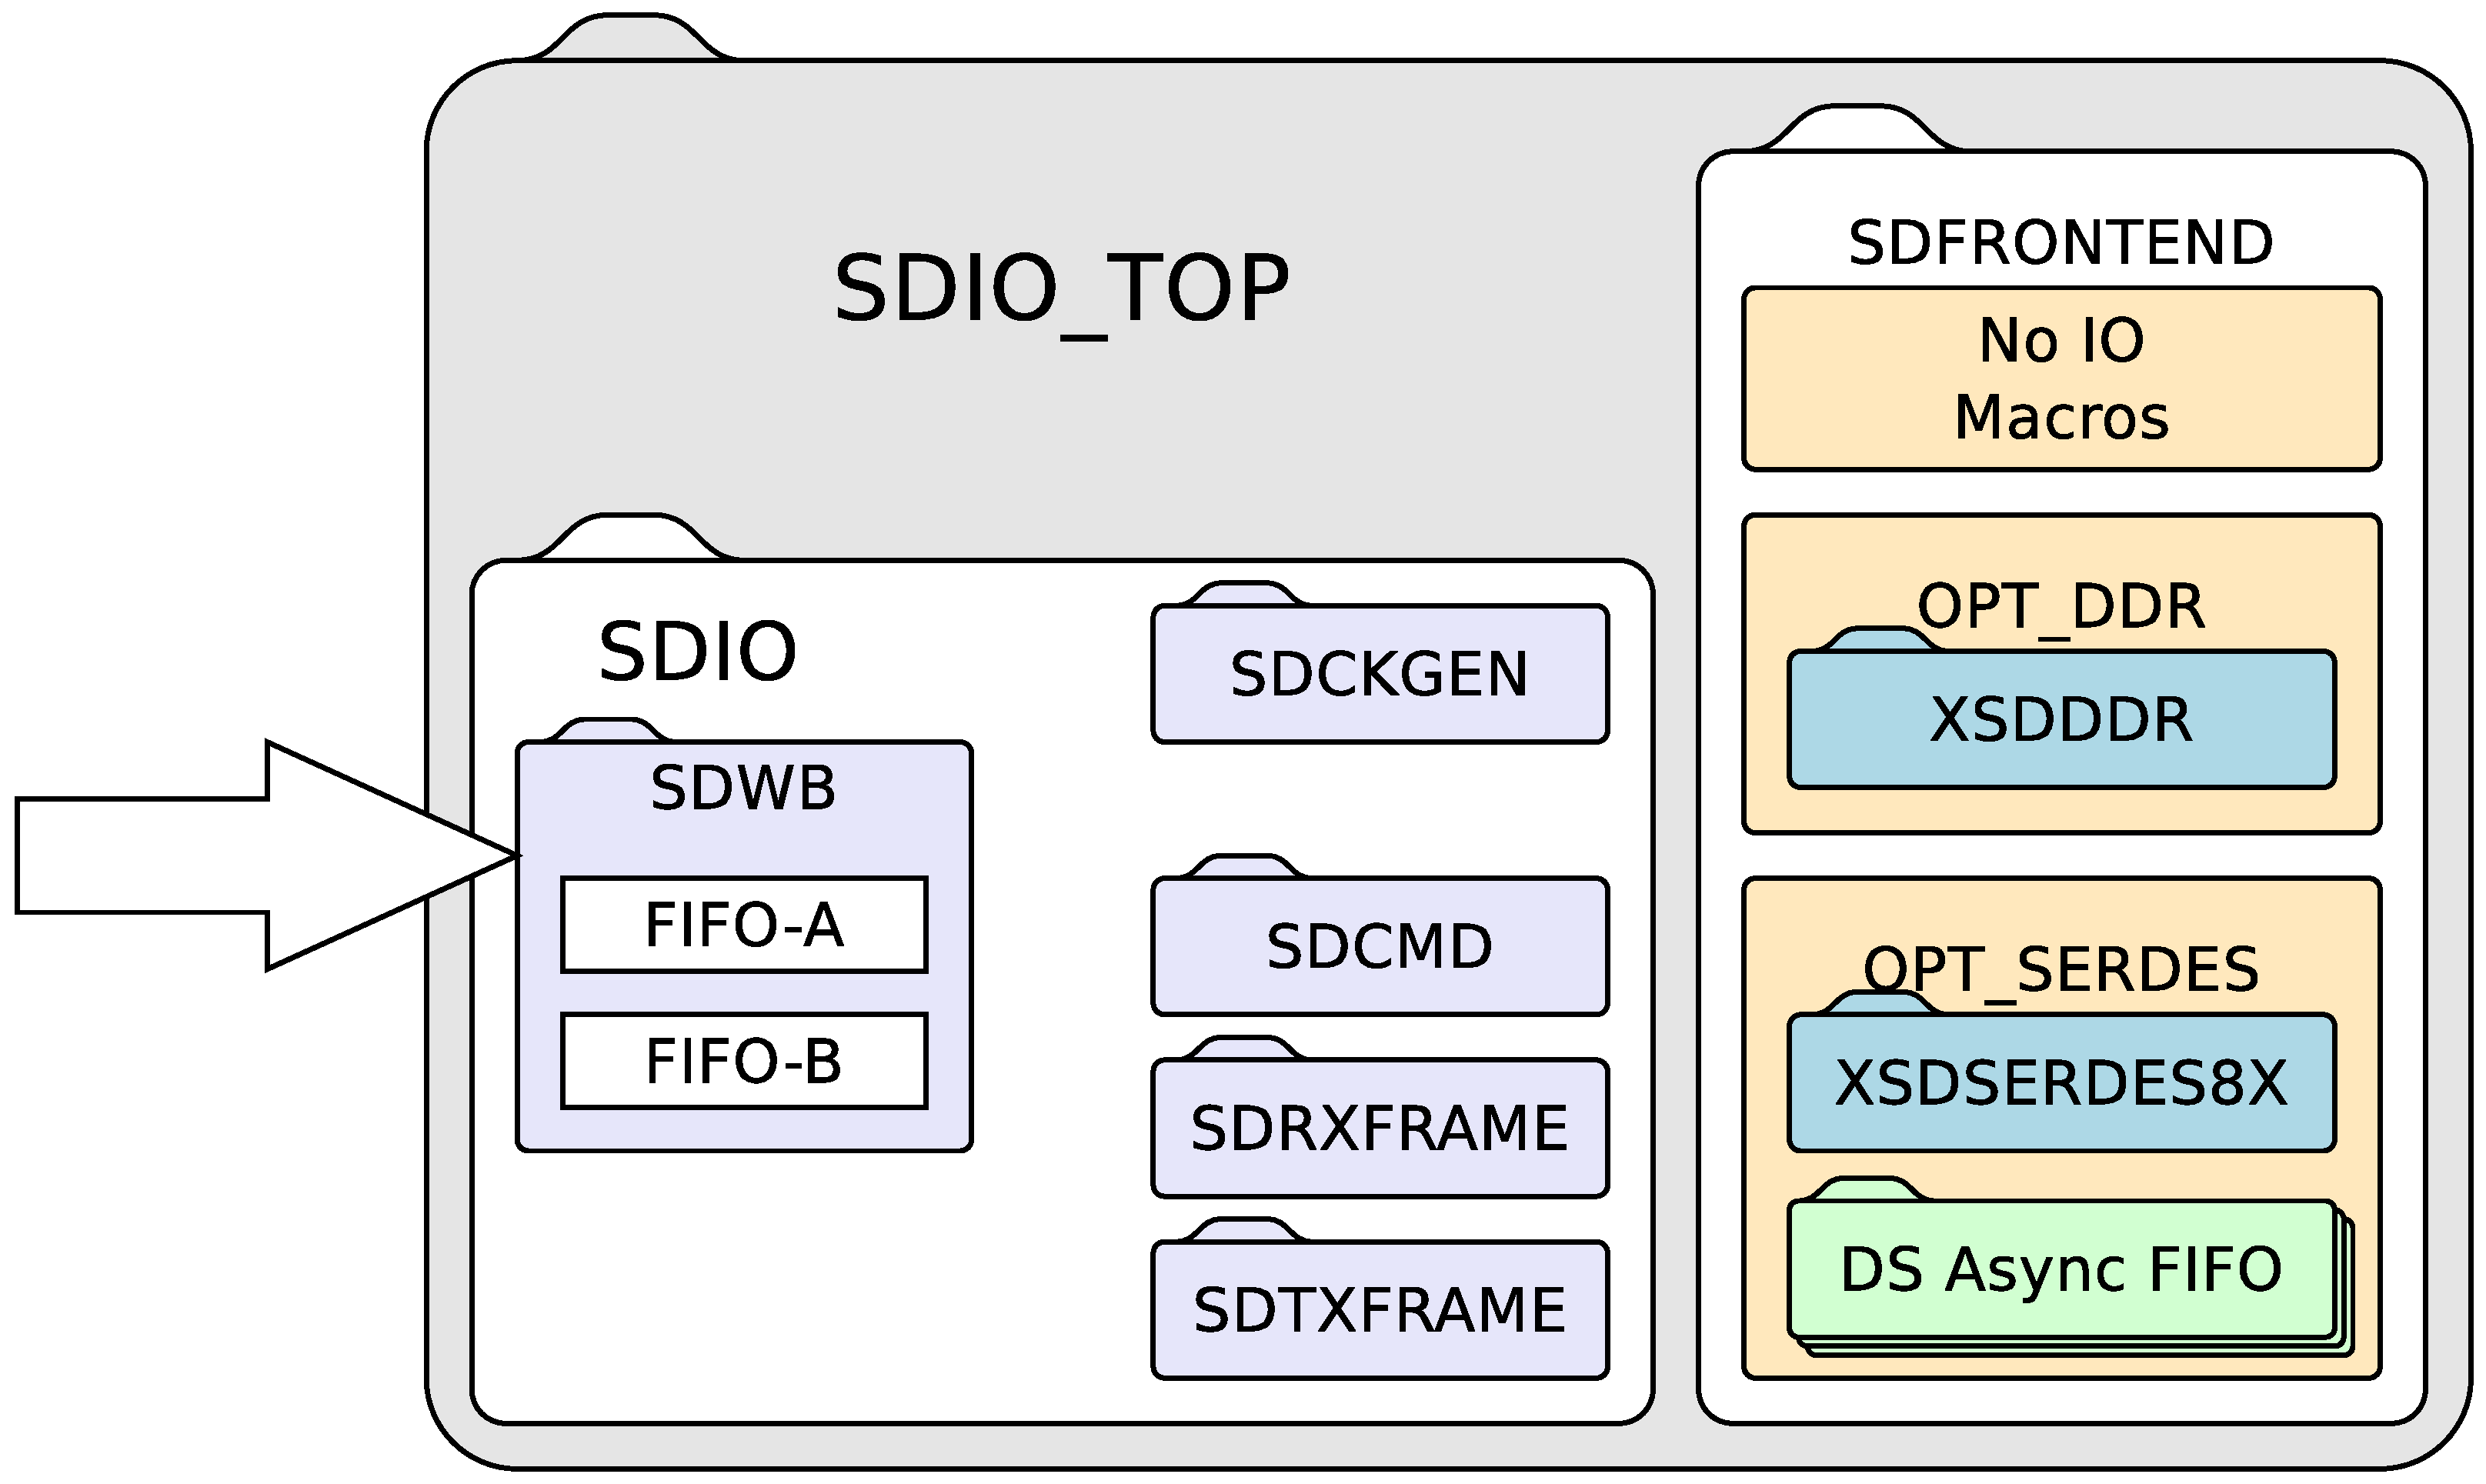
\includegraphics[height=2.5in]{gfx/sdioblocks.eps}
\caption{SDIO/eMMC Controller RTL Architecture}\label{fig:sdioblocks}
\end{center}\end{figure}
The design is broken up into two parts at the top level: a hardware independent,
all digital logic component whose top level is \zhref{../rtl/sdio.v}{\tt sdio.v},
and a hardware dependent front end component whose top level is found in
\zhref{../rtl/sdfrontend.v}{\tt sdfrontend.v}.

The core controller, found in \zhref{../rtl/sdio.v}{\tt sdio.v}, itself is
composed of five separate components.  The first,
\zhref{../rtl/sdwb.v}{\tt sdwb.v}, is the controller.  This component is
a wishbone slave.  All user interaction goes through this controller.
Requests for transfers are made here.  Data to be transferred is stored here
in one of two FIFOs for transmission to the front end.  Data to be received
is stored here after reception, to be read out as it becomes available to the
CPU.  Even when using the DMA, data will first be stored in the FIFO's within
the controller before going to the card, or after coming from the card.

A second, alternative, controller implementation exists in
\zhref{../rtl/sdaxil.v}{\tt sdaxil.v}.  This controller is nearly line for line
identical to the \zhref{../rtl/sdwb.v}{\tt sdwb.v} controller, save that
interaction with this controller takes place over AXI instead of Wishbone.

The controller maintains a PHY register for configuring the front end.  This
register also controls the clock generator, \zhref{../rtl/sdckgen.v}{\tt sdckgen.v}.  This clock
generator is responsible for generating the clock used throughout the
interface.  That clock is internally represented as an 8-bit vector, allowing
it to specify zero, one, or up to two clock periods, each either aligned with
or 90 degrees offset from the data, per 8-bits.  This clock may also be divided
to slower speeds as requested by the user.  Finally, a user setting allows the
clock to turn off when it isn't being used, to save on interface power and
to potentially reduce emissions.  (Note that this only turns off the IO clock,
not any of the system clocks used throughout the design to clock the logic
within the design.)  Turning off the clock may be required when working with
the multiblock read command, to ensure that the FIFO is properly cleared before
subsequent blocks are read.

Commands issued to the controller will be forwarded to the \zhref{../rtl/sdcmd.v}{\tt sdcmd.v}
module.  This module is responsible for all interactions taking place over
the CMD wire.  The module can generate 48-bit commands, beginning with a
start bit and ending with a CRC and a stop bit.  It can then recognize
either 48-bit or 136-bit command responses.  Responses are checked against
both the CRC and frame errors.  If the device fails to return a response
within a given timeout window, the response may also timeout with an error,
after which the command controller will no longer expect any response until
the next command is sent.

Fig.~\ref{fig:sdcmdflow}
\begin{figure}\begin{center}
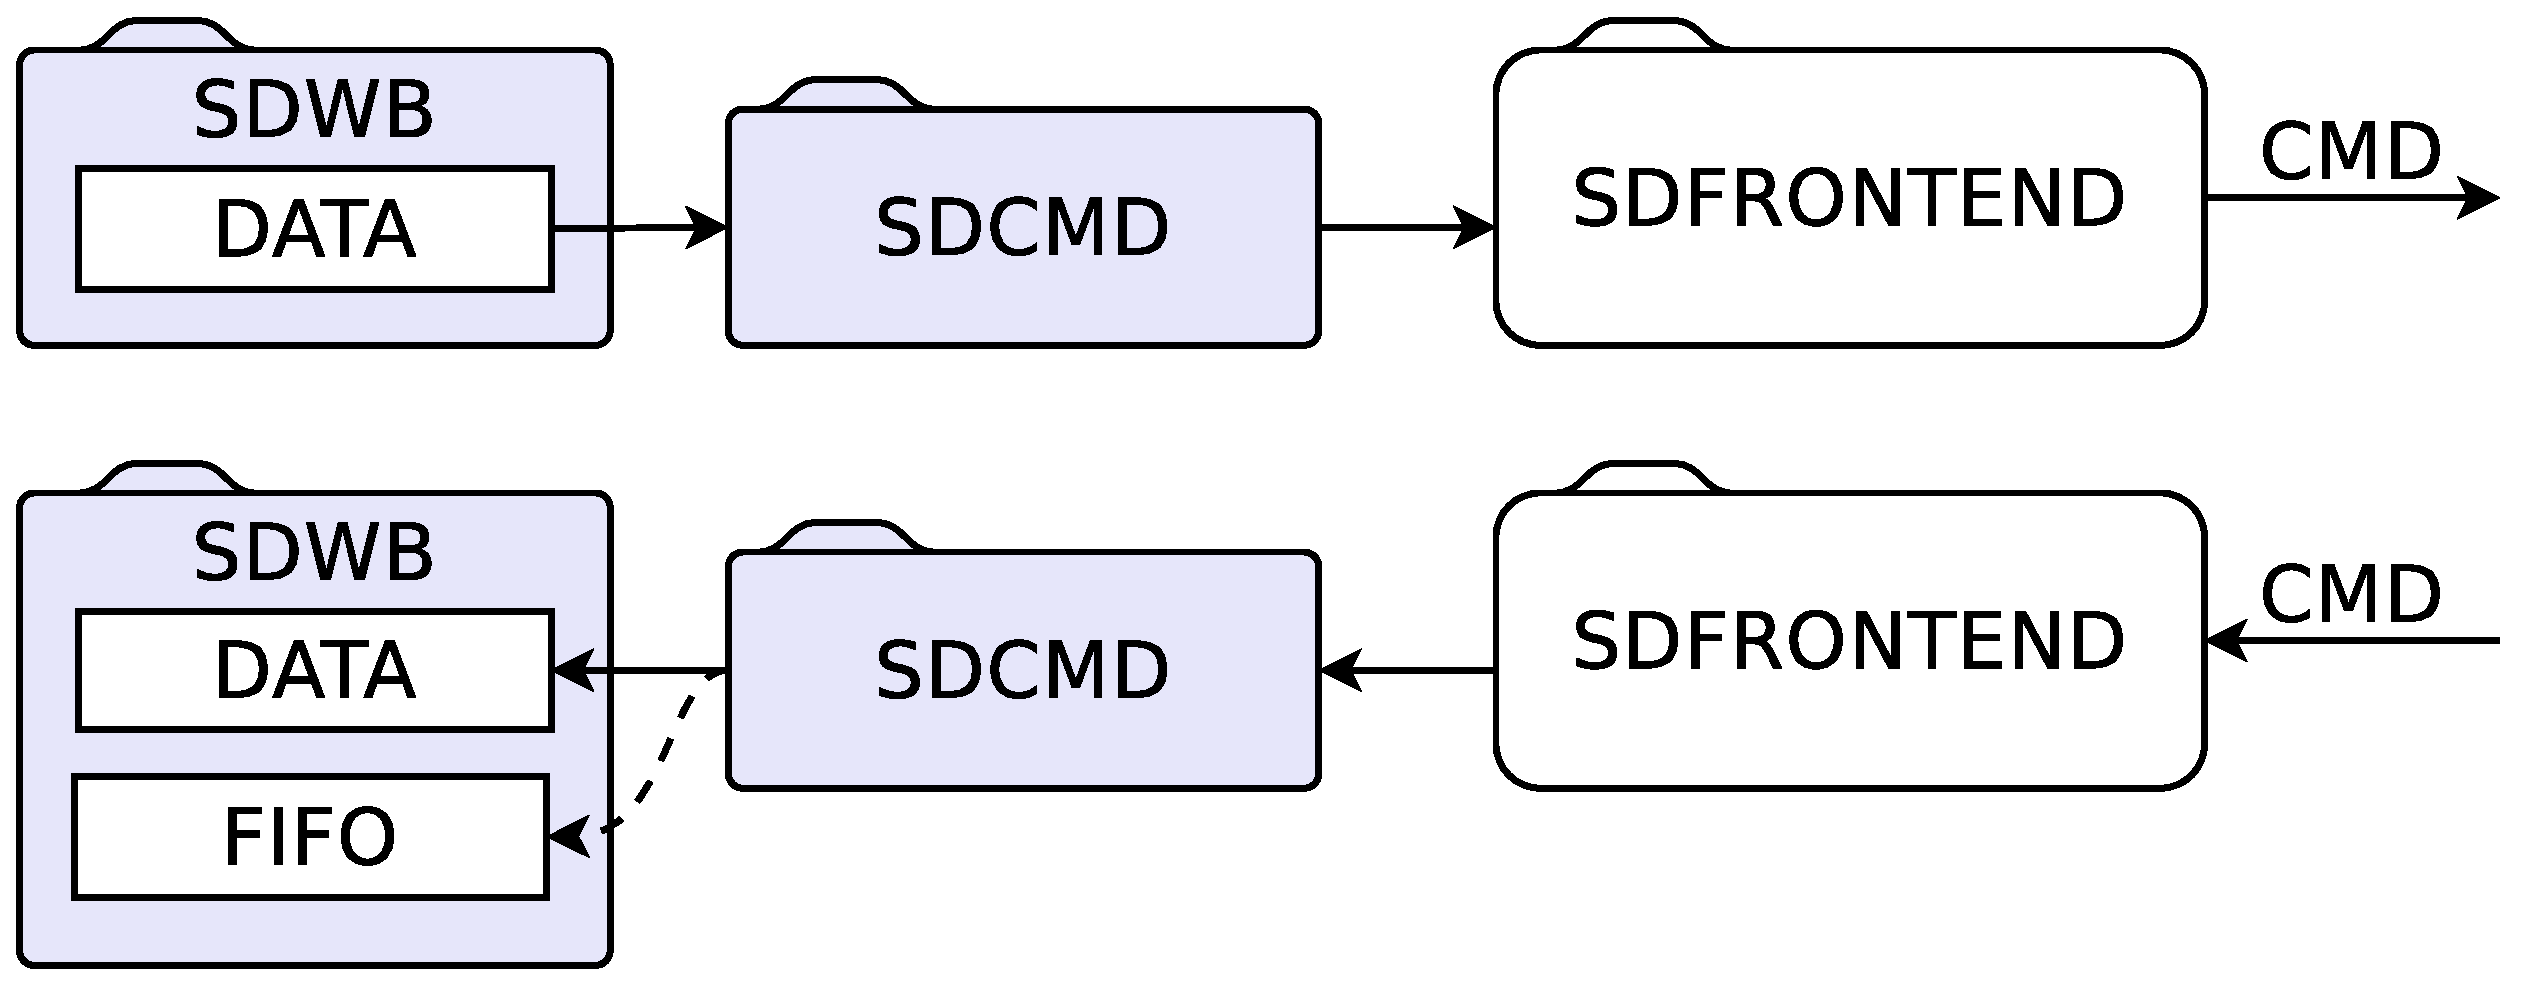
\includegraphics[width=5.0in]{gfx/sdiocmdflow.eps}
\caption{SDIO/eMMC CMD pin data flow}\label{fig:sdcmdflow}
\end{center}\end{figure}
shows both the basic command flow, and the two possible response flows.
For commands, a data register within \zhref{../rtl/sdwb.v}{\tt sdwb.v} is first set, then the
command is issued.  The \zhref{../rtl/sdcmd.v}{\tt sdcmd.v} module organizes both into a 48-bit
word to be transmitted.  The \zhref{../rtl/sdcmd.v}{\tt sdcmd.v} module then looks for one of
two responses, either a 48--bit response which would place the 32-bit
argument back in a data register, or a 136--bit response which would be
placed into one of the two FIFOs in \zhref{../rtl/sdwb.v}{\tt sdwb.v}.

One type of controller command is a memory command.  These commands send a
48-bit command to the device, followed by sending data to or receiving data
from the device.

The \zhref{../rtl/sdrxframe.v}{\tt sdrxframe.v} component is activated when data is expected from the
device on the data wires.  It's purpose is to collect the data returned from
the front end controller, and re-form that data into commands to write to
one of the FIFOs in \zhref{../rtl/sdwb.v}{\tt sdwb.v}.  If a full frame, as defined by the
controller, is not received prior to a timeout, or if a CRC error is detected
within that frame, the receive component will report an error and give up
in order to wait for its next command.

Similarly, the \zhref{../rtl/sdtxframe.v}{\tt sdtxframe.v} command is activated when data is to be
sent over the data wires to the device.  In this case, data flows from one
of the FIFOs in \zhref{../rtl/sdwb.v}{\tt sdwb.v} to \zhref{../rtl/sdtxframe.v}{\tt sdtxframe.v}, gets formatted for the
front end to output, a start bit, CRC, and stop bit are added, and all get
sent to the front end.  This basic flow is shown in Fig.~\ref{fig:sdiotxflow}.
\begin{figure}\begin{center}
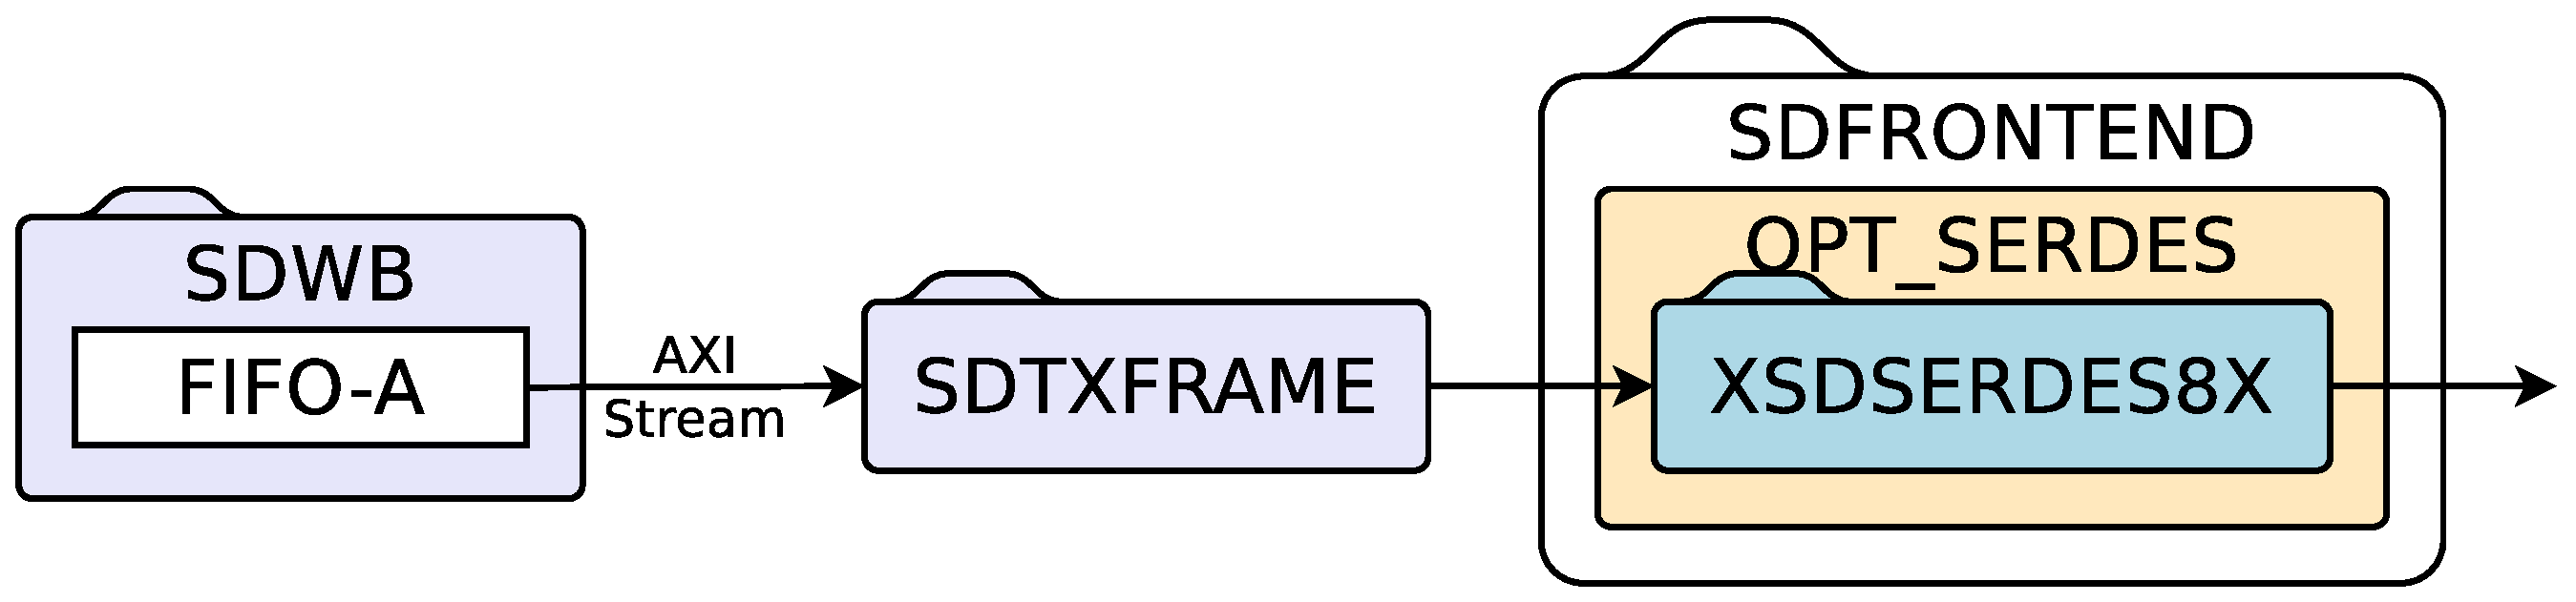
\includegraphics[width=5.0in]{gfx/sdiotxflow.eps}
\caption{SDIO/eMMC transmit data flow, to the device}\label{fig:sdiotxflow}
\end{center}\end{figure}
When controlling an eMMC device, the
\zhref{../rtl/sdtxframe.v}{\tt sdtxframe.v} transmit component can also be
configured to expect and wait for a CRC token acknowledging a successful
transfer.  This is an eMMC only feature.

Let's now turn our attention to the device dependent front end.

The front end was initially defined for full IO support, all the way up to
HS400 and the eMMC data strobe.  Driven from a 100~MHz clock, this means that
this front end was designed to support up to two device clock periods per
100~MHz system clock, and to have data sent on each edge of these two clock
periods.  This forces a requirement of 4-data bits output per 100~MHz system
clock cyle per data pin.
The clock, however, also needs to be (potentially) offset by 90~degrees from
that data.  As a result, all I/O using this particular front end capability,
called the {\tt OPT\_SERDES} capability in Fig.~\ref{fig:sdioblocks}, takes
place using Xilinx's 8:1 OSERDES elements.  Incoming bits are either sent
to an asynchronous FIFO, to support the eMMC data strobe, or they are
sampled via 1:8 ISERDES elements.  In the case of the ISERDES inputs, sample
timing is controlled via both the output clock rate, as well as a user
controlled digital delay, allowing sample alignment with clock precision
of one eighth of a system clock.  Hence, even without the full speed HS200
support, this subsample re-alignment may still be quite valuable when supporting
higher speeds.  All Xilinx specific SERDES interactions are captured in an
\zhref{../rtl/xsdserdes8x.v}{\tt xsdserdes8x.v} module.

Logic resources throughout the design may be reduced, however, by switching
to a simpler front end architecture.  Two other architectures are available:
the {\tt OPT\_DDR} architecture and a plain architecture that doesn't use
any IO macros--save for the {\tt IOBUF} macro used for controlling any
tristate capabilities.

The {\tt OPT\_DDR} architecture is roughly the same as the {\tt OPT\_SERDES}
architecture, save the DDR IO elements are used to generate both clock and
data instead of the SERDES elements.  This should make it possible to drive
the IO pins at the full clock speed using SDR, or at half the clock speed
using DDR.  In this case, all Xilinx specific IDDR and ODDR interactions are
captured in an \zhref{../rtl/xsdddr.v}{\tt xsdddr.v} module.

The no macro architecture was built in order to support an architecture
where the {\tt SD\_CK} pin was routed through the Xilinx {\tt CCK} pin,
and hence through an {\tt STARTUPE2} primitive.  In this case, no IO macros
are available for controlling the clock, and all IOs are controlled directly
from logic.  The fastest clock this architecture can generate is half the
system clock rate.

These constitute the basic components of the controller, both hardware
independent and hardware dependent.
%% }}}
\section{DMA Architecture}\label{sec:arch-dma}
%% {{{
The DMA is built from several parts.  The first key component to the DMA is
found in the control module, \zhref{../rtl/sdwb.v}{\tt sdwb.v}.  The controller
is responsible for sectioning transfers into per-block requests, and forwarding
data to and from the DMA module itself.  The rest of the DMA logic is found
in the DMA module, \zhref{../rtl/sddma.v}{\tt sddma.v}.  This module is shown
in Fig.~\ref{fig:dmablocks}.
\begin{figure}\begin{center}
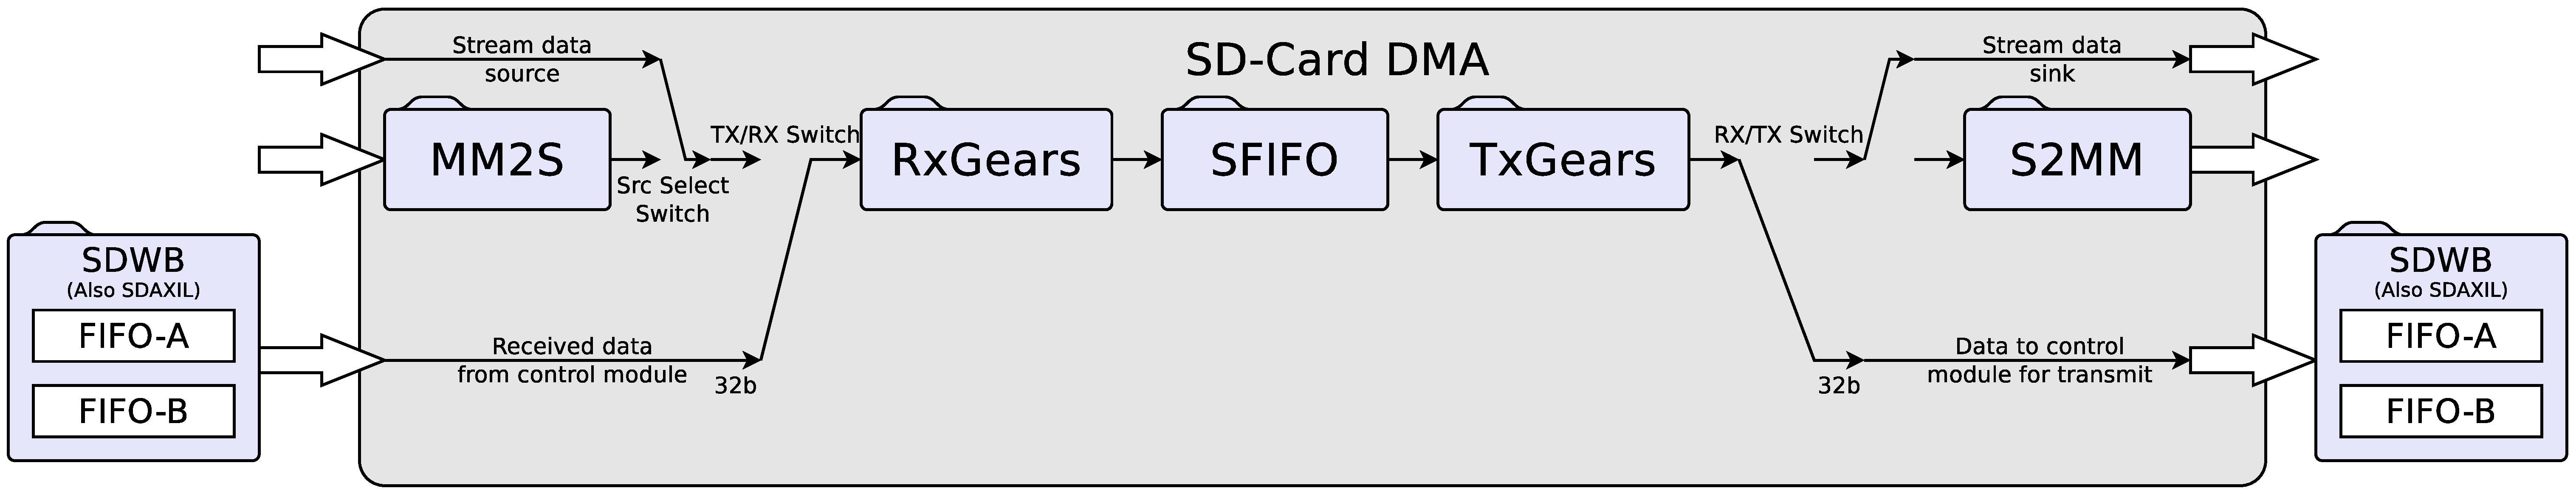
\includegraphics[width=5.0in]{gfx/dmablocks.eps}
\caption{DMA Block Diagram}\label{fig:dmablocks}
\end{center}\end{figure}

When using the DMA, data continues to go through the FIFOs in the controller
module just as it would without the DMA present.  The difference is that these
FIFOs will be automatically sourced from, or emptied into, a DMA module which
will then handle copies
from, or to, memory.  Hence, for a write operation, the user will request
the write operation and then the controller will tell the DMA to supply data
for one of its FIFOs.  Once the FIFO is filled, the controller will send it
to the external device.  Then, while the data is being transmitted to the
device, the controller will continue to request source data capture to supply
any subsequent data transfer requirements.  Likewise, for a read operation,
the user will request the operation first, followed by a block getting
transferred to the controller's FIFO.  The read will then continue filling
the second FIFO will the first one is drained by the DMA.  If both FIFO's
fill faster than the DMA can empty them when reading from the device, then
the IO clock will be stopped to wait for the next FIFO to be drained.

That's a high level overview, from the perspective of a DMA enabled control
module.  Let's now turn our attention to how the DMA supplies and deals
with the data streams given to it.

Data arrives in the DMA module from one of three sources.  First, if both
{\tt OPT\_ISTREAM} and the MSB of the DMA address are set, data may arrive from
an AXI stream.  If used, this most-significant bit is one wider than the
address width of the devices bus.  Alternatively, data may be read from memory
using the \zhref{../rtl/sddma\_mm2s.v}{\tt sddma\_mm2s.v} (or
\zhref{../rtl/sdax\_mm2s.v}{\tt sdax\_mm2s.v}) component.  Finally, when reading
from the card, data will arrive first in the controller module, and then be
forwarded from it once the respective buffer is full.

These sources may have different data widths.  Data arriving from memory will
arrive packed in bits that may be up to the full bus width in size.  Data
arriving from the controller will always be 32b wide.  Data arriving from the
stream port may be either of these widths.  The receiving gearbox,
\zhref{../rtl/sddma\_rxgears.v}{\tt sddma\_rxgears.v}, will therefore take this
data stream and pack it into beats at the widest of these widths.

From here, data enters into a FIFO.  This guarantees that the memory source
never needs to stall, or otherwise provide backpressure on the bus--something
not supported by the Wishbone interface.  The FIFO also allows data to arrive
at wide widths, only to be read at slower (32b) rates if necessary.

From the FIFO, the data width is adjusted in the transmit, or outgoing,
gearbox, \zhref{../rtl/sddma\_txgears.v}{\tt sddma\_txgears.v}.  This component
optionally adjusts the data width back down to 32b if required.  Either the
stream output, or the controller interface may require this width.  If going
back to memory, the width will be left at the full size of the bus.

The final step in the DMA process is to forward the data stream to one of
three ultimate destinations.  When writing to the card, the ultimate
destination will send the data to the controller.  When reading from the card,
data may either be written to memory or to the AXI stream interface.  The AXI
stream interface will be used when/if both {\tt OPT\_OSTREAM} is set and
the most significant address bit are set.

A small amount of logic exists in the \zhref{../rtl/sddma.v}{\tt sddma.v}
module to control the switching between sources and outputs, as well as to
make sure block boundaries are respected.
%% }}}
\section{Verification Architecture}\label{sec:arch-vip}
%% {{{
The verification architecture is built around a model of the
downstream device.  One such model is shown in Fig.~\ref{fig:mdlsdio}.
\begin{figure}\begin{center}
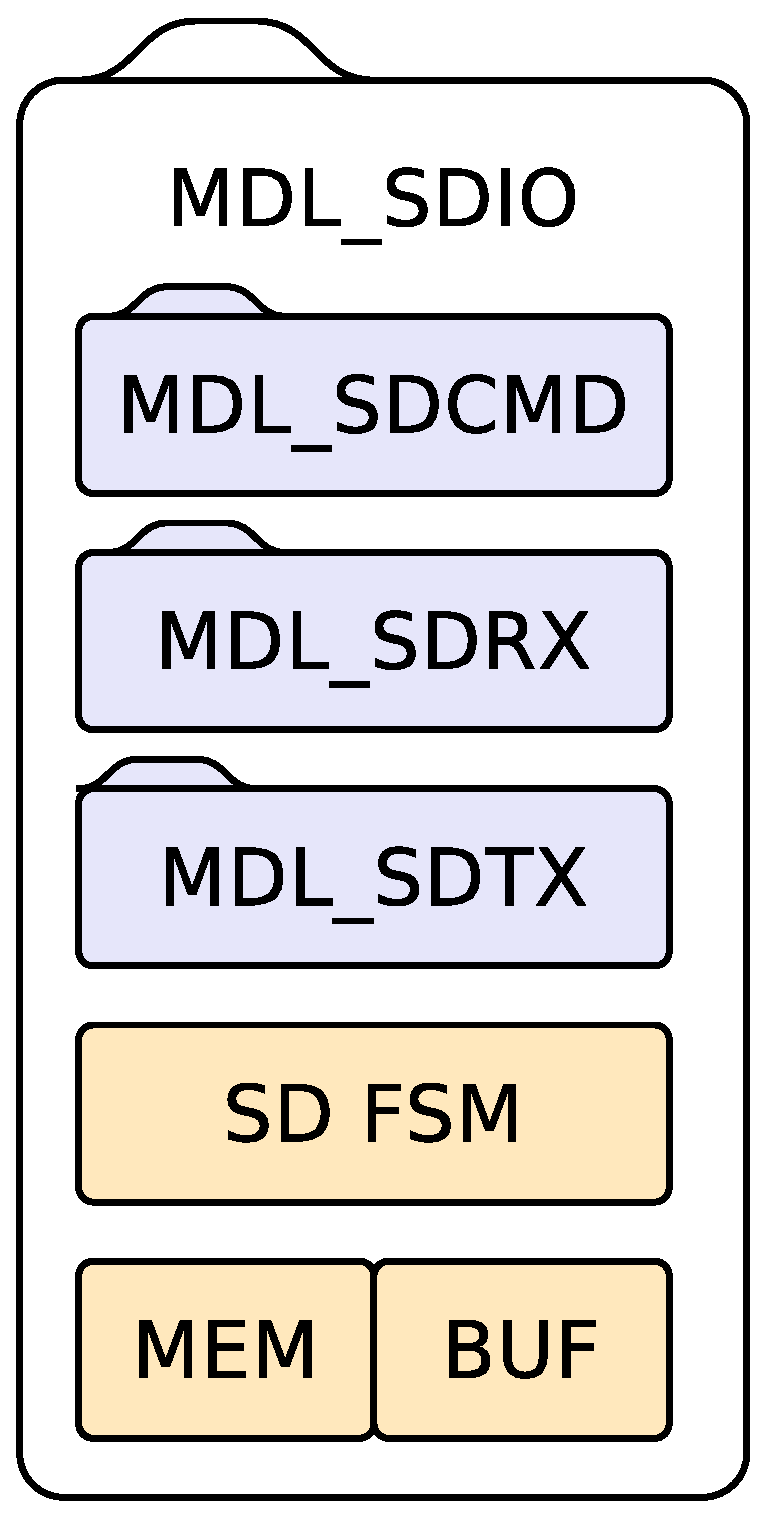
\includegraphics[height=2.5in]{gfx/mdlsdio.eps}
\caption{SDIO Verification IP}\label{fig:mdlsdio}
\end{center}\end{figure}
A second, similar, Verilog model exists for modeling the eMMC interface.
These Verification IP modules contains full featured submodules for handling
the command wire, receiving data, and transmitting data.  These three
submodules are designed to correspond to their host controller counterparts.
Further, these three submodules have been built to be independent of whether
the controller is modeling an SDIO or an eMMC interface.

The smarts of this Verfication IP (VIP) are found in the finite state machine
(FSM) at the top level of \zhref{../bench/verilog/mdl\_sdio.v}{\tt mdl\_sdio.v}.
This state machine responds to commands, and generates responses to them.  A
data transfer buffer exists for sending or receiving data across the interface.
A second memory within the VIP, shown as {\tt MEM} in Fig.~\ref{fig:mdlsdio},
captures the persistent memory found in the SDIO (or eMMC) device.

The entire Verilog test bench infrastructure is diagrammed in
Fig.~\ref{fig:vlogtb}.
\begin{figure}\begin{center}

\includegraphics[width=5.0in]{gfx/vlogtb.eps}
\caption{Test-bench infrastructure block diagram}\label{fig:vlogtb}
\end{center}\end{figure}
In this setup, a test script drives a Wishbone Bus Functional Model (BFM).
The BFM issues 32b bus requests, which are then resized to the full width
of the bus.  From here, requests go into a crossbar, and get routed to either
an SDIO (via a width downsizer), an eMMC controller (via a width downsizer),
a block RAM model (at the full bus width), a console port, a GPIO port,
or a stream checking controller.  This then allows the test
script to interact with the IP, which then drives interactions with one of the
two backend VIP device models.  If the DMA's are present, they can also be used
to transfer data to or from the RAM via the bus interconnect.  If the stream
option has been enabled, the stream checker can be used to both generate
stream data and to verify that incoming data matches what had been generated.
What tests get accomplished at this point is then dependent upon the test
script.  Two test libraries are also available,
\zhref{../bench/testscript/sdiolib.v}{one for SD cards} and
\zhref{../bench/testscript/emmclib.v}{one for eMMC cards}.  These
libraries help define common constants and supporting common test script tasks
which can be called by the test script itself.

Two versions of this top-level interface exist.  The first supports
all Wishbone interactions.  It can be found in
\zhref{../bench/verilog/tb\_wb.v}{\tt tb\_wb.v}.  A second top level exists for
testing AXI interactions.  This is found in
\zhref{../bench/verilog/tb\_axi.v}{\tt tb\_axi.v}.

\iffalse
A third test bench infrastructure, shown in Fig.~\ref{fig:cputb},
\begin{figure}\begin{center}
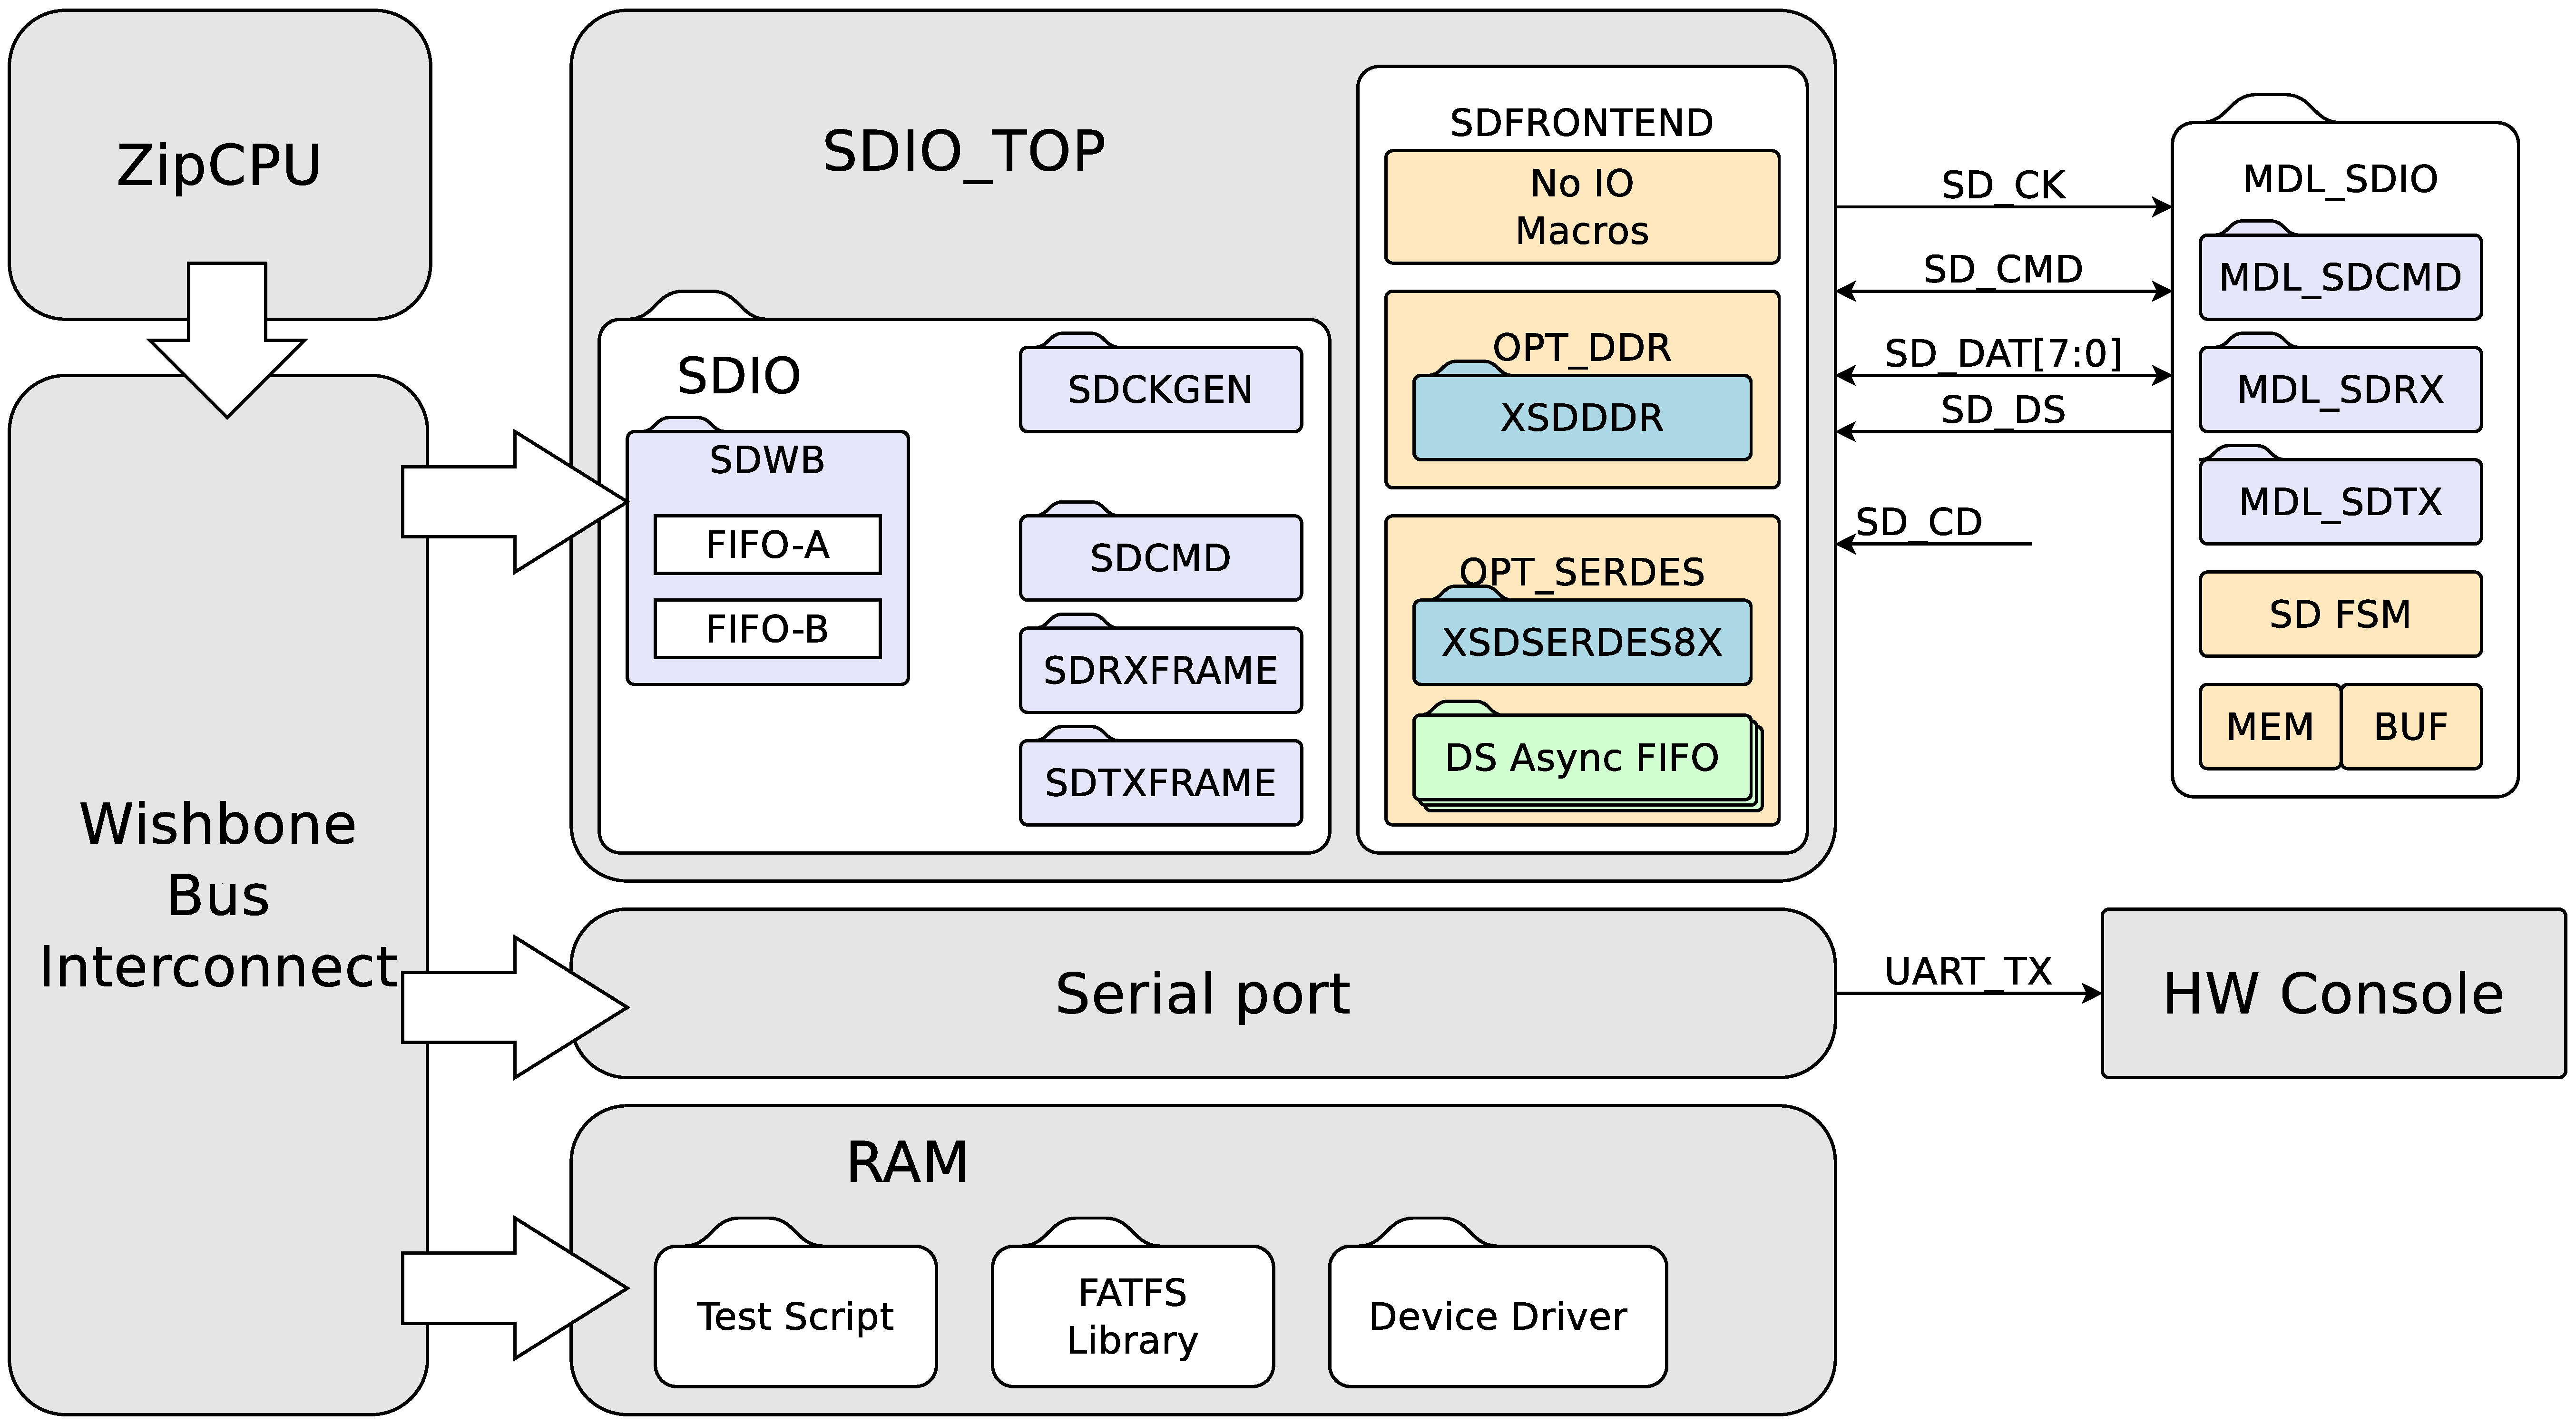
\includegraphics[width=5.0in]{gfx/cputb.eps}
\caption{All Verilog top-level model}\label{fig:cputb}
\end{center}\end{figure}
is also envisioned.  This infrastructure will contain a soft--core ZipCPU,
a serial console, and memory.  In this test architecture, the test script
exists as a software program supported by both the
\zhref{http://elm-chan.org/fsw/ff/}{FATFS} library and the
software driver.  Once complete, the purpose of this testbench infrastructure
will be to specifically test and verify the software driver in its native
(software) form, compiled for and then running on a soft--core CPU.  In this
case, that softcore CPU will be the ZipCPU.
\fi
%% }}}
\section{Software Driver Architecture}\label{sec:arch-swdrvr}
%% {{{

At present, there exist three software drivers and one glue layer for each.
The three drivers are found in the \zhref{../sw/}{\tt sw/} directory.  These
respective drivers are:
\begin{itemize}
\item \zhref{../sw/sdspidrv.c}{\tt sdspidrv.c}: A software driver for the SPI
	version of this controller.  The SPI version of this controller is
	described in the SDSPI user guide.
\item \zhref{../sw/sdiodrv.c}{\tt sdiodrv.c}: A software driver for the SDIO
	controller, described in this user guide.  This controller is designed
	to interact with an SD Card.
\item \zhref{../sw/emmcdrv.c}{\tt emmcdrv.c}: A software driver for the eMMC
	controller.  This is designed to interact with the same SDIO/eMMC
	controller discussed in this user guide.  However, the SDIO and eMMC
	protocols require different commands to interact with their respective
	devices.  As a result, in spite of any similarities, the eMMC software
	driver differs significantly from the SDIO software driver.
\item \zhref{../sw/diskiodrvr.c}{\tt diskiodrvr.h} provides a common definition
	of a device ``driver'', which can be used across all of the device
	drivers listed above.

	More on this in a moment.
\item \zhref{../sw/diskio.c}{\tt diskio.c} is a shared/common dispatch glue
	layer.  Commands from the \zhref{http://elm-chan.org/fsw/ff/}{FATFS}
	subsystem naturally land here, where they are then dispatched to the
	appropriate controller.
\end{itemize}

Put together, this IO subsystem has the various layers shown in
Fig.~\ref{fig:swlayers}.
\begin{figure}\begin{center}
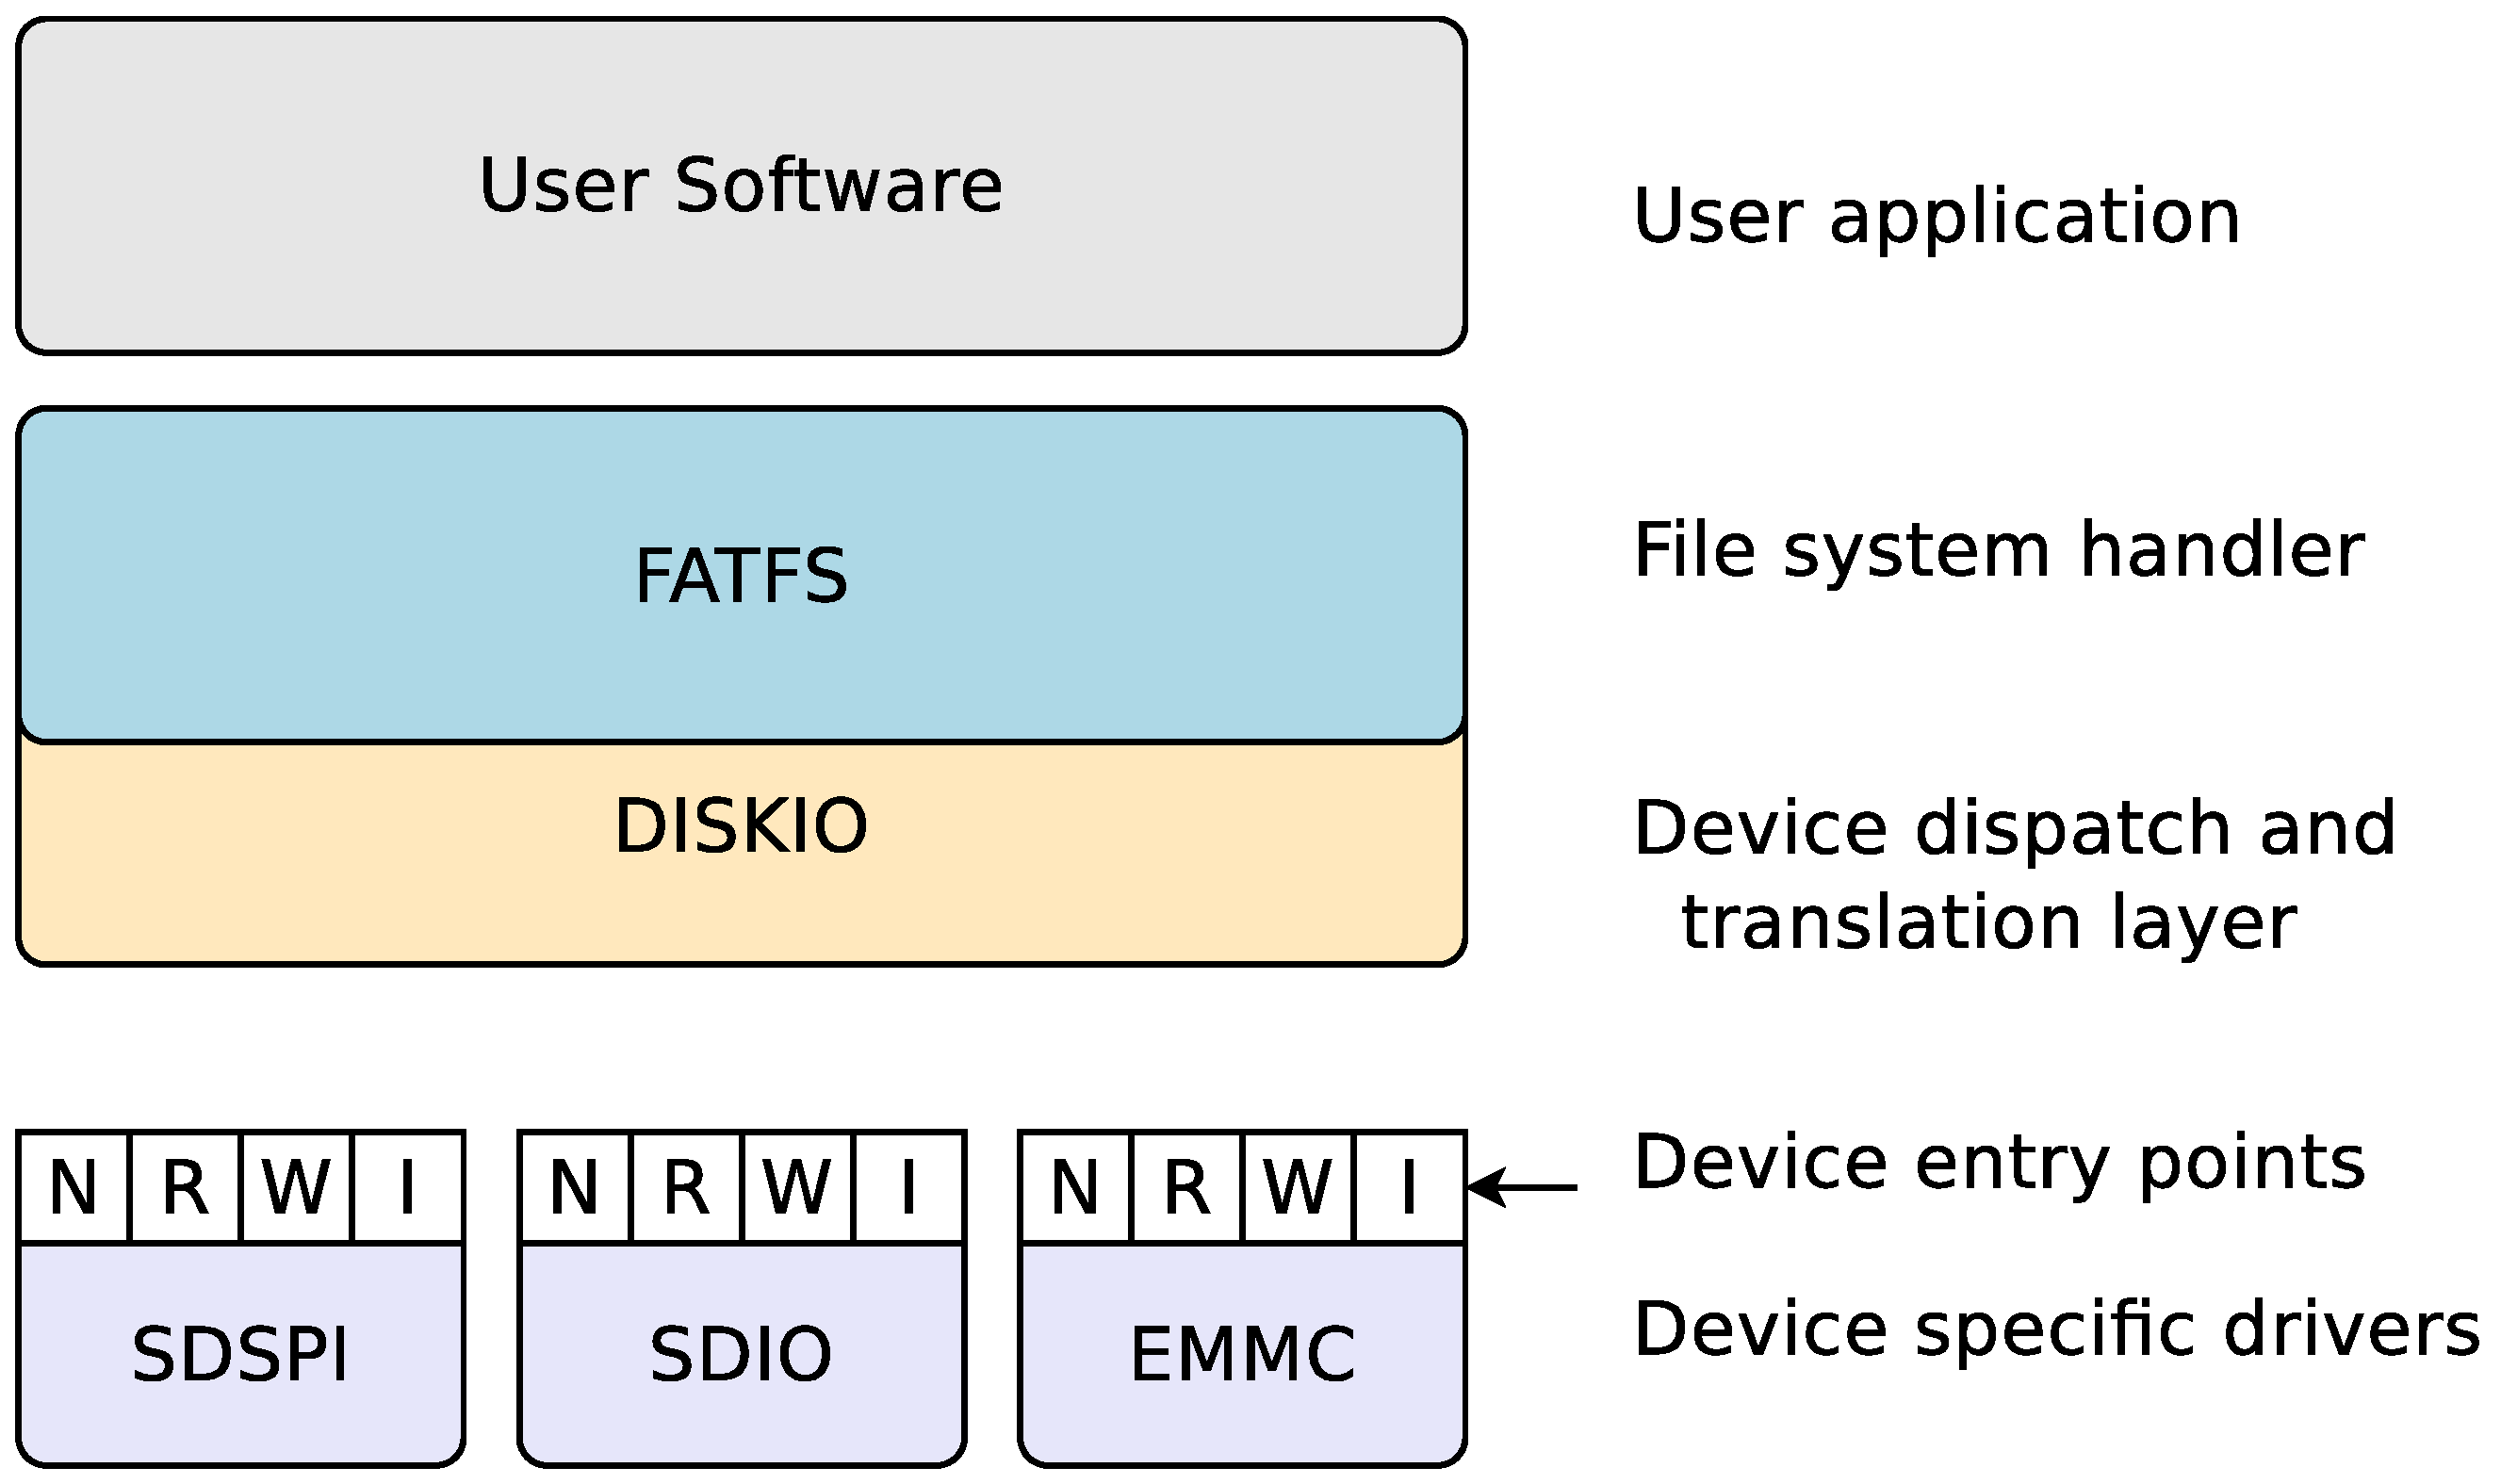
\includegraphics[height=2.5in]{gfx/swlayers.eps}
\caption{Software Stack}\label{fig:swlayers}
\end{center}\end{figure}
User software interacts with the \zhref{http://elm-chan.org/fsw/ff/}{FATFS}
layer.  \zhref{http://elm-chan.org/fsw/ff/}{FATFS} then interacts with the
device dispatch layer.  The device dispatch layer then instantiates and
interacts with one (or more) of the device drivers beneath it.

Each device driver has four entry points--``methods'' in Object Oriented
terminology.  The first method is used to initialize the driver and set up
its data structures.  After that, there are methods for reading and writing.
Finally, there's an IOCTL method which can be used for other tasks such as
querying the size of the device or the size of a data block.
%% }}}

%% }}}
\chapter{Operation}\label{ch:ops}
%% {{{
At its most basic level, interacting with the controller simply involves
configuring the PHY, setting the data you wish to send, and then sending a
command to the controller.  This needs to take place, however, in many
different contexts.  Some commands don't expect responses, whereas others
return 48 or even 136--bits.  Some commands are followed by data transmission,
whereas others do not.  This section therefore walks through several
examples of commands, illustrating the range of commands and responses
that can be issued using this controller.

\section{Waiting for a card}
%% {{{
Prior to a card being inserted in the slot, the design will be held in
reset.  Hence the first important step when working with an SD card is to
wait for the SD card to be present.
\begin{zCpp}
	const	unsigned	SDIO_PRESENTN  = 0x00080000;
	unsigned	cmd;

	do {
		cmd = _sdio->sd_cmd;
	} while(cmd & SDIO_PRESENTN);
\end{zCpp}

Once an SD card is present, as part of the initialization process, the first
step is then to acknowledge it.
\begin{zCpp}
	const	unsigned	SDIO_NULLCMD  = 0x00000080,
				SDIO_REMOVED  = 0x00040000;

	_sdio->sd_cmd = SDIO_REMOVED | SDIO_NULLCMD;
\end{zCpp}

If this bit is ever set from here on out, it will indicate that the SD card
has been removed.  If the command register indicates a card is present, yet
the removed flag is still high, it may be that a card was removed and a
new one inserted.  Either way, the controller may will need to restart the
card with a {\tt GO\_IDLE} command.

%% }}}
\section{Querying PHY Capability}
%% {{{
It can be important to know how the device was configured, so let's continue
there next.  Specifically, let's start by trying to determine which version of
the PHY is present.  We can do this by requesting a 200~MHz clock, an 8~bit
bus width, DDR mode, and a full PHY shift.  We'll also allow the device to
turn the clock off when not in use, so we that we don't push a high
speed clock accidentally before the device has been properly configured
for it.

\begin{zCpp}
	const	unsigned	SDIOCK_200MHZ = 0x00000000,
				SDPHY_W4      = 0x00000400,
				SDPHY_WTEST   = 0x00000c00,
				SDPHY_DS      = 0x00004300,
				SDPHY_DDR     = 0x00004100,
				SPEED_CLKOFF  = 0x00008000,
				SDPHY_SHFTMSK = 0x001f0000,
				SECTOR_MAX    = 0x0f000000;
	unsigned	phy;

	_sdio->sd_phy = SDIOCK_200MHZ | SDPHY_WTEST | SDPHY_DDR
			| SDPHY_SHFTMSK | SPEED_CLKOFF | SECTOR_MAX;
	while(3 < (phy = _sdio->sd_phy & 0x0ff))
		;
\end{zCpp}

As always, whenever changing the clock speed, it's important to wait for
the change to complete.  Notice, though, that we aren't waiting for the
clock to reach 200~MHz.  Instead, we wait until the clock is at least 25~MHz.
This is because not all front ends can support the 200~MHz clock.  Therefore,
we wait for the clock rate to change, and then see which clock rate we have.

We can now examine the \cppinline{phy} return value to learn our configuration.
\begin{itemize}
\item If \cppinline{0 == (phy & SDPHY_WTEST)}, then we know the controller will
	only support a single data bit.  If
	\cppinline{SDPHY_W4 == (phy & SDPHY_WTEST)}, then we know it will
	support either 1 or 4 data bits.  Otherwise, the PHY will support
	an 8~bit interface--useful for eMMC devices.

\item The \cppinline{SDPHY_SHFTMSK} specifies 5 bits of a shift register
	which can be used to control where return sampling takes place.  If
	the all bits remain set in \cppinline{phy}, then design was built
	with the SERDES front end.  If the all but the bottom two bits are
	set, then the DDR front end has been built, etc.

	Depending upon which version of the PHY is available, the sample
	shift may need to be adjusted.  Beware, though, that this may be
	a board specific setting.

\begin{zCpp}
	unsigned	sample_shift = 0;

	// Shift amounts shown are only notional, and may (or may
	// not) reflect the appropriate values for your hardware.
	if (phy & 1) {
		// SERDES PHY
		sample_shift = 9 << 16;
	} else if (phy & 4) {
		// DDR PHY
		sample_shift = 16 << 16;
	} else
		sample_shift = 24 << 16;
\end{zCpp}


\item The clock frequency returned indicates the fastest clock rate the design
	can operate in DDR mode.  Often, the design can go one speed step
	faster in a non--DDR mode, but this is still useful as a starting
	point.

	For example, the DDR PHY can handle SDR104 (a 100MHz clock) when
	operated from a 100MHz system clock.  This would have a clock setting
	of \cppinline{1 == (phy & 0x0ff)}.  However, DDR requires a 90 degree
	clock offset from the data, and achieving this offset will force
	the maximum speed to be \cppinline{2 == (phy & 0x0ff)} (50~MHz or
	DDR50).

\item If the DS bit is set, \cppinline{(phy & 0x0200)}, then the PHY can
	support return data strobe handling.

\item Finally, the PHY register will indicate the maximum sector size
	available to it--typically 512Bytes, but it might be larger.
	This size is given by \cppinline{sz = (1 << ((phy>>28)&0x0f));}.
\end{itemize}

A similar approach may be used to determine if the DMA is present.  We can
start by writing a negative one to the length register, and then reading
the result back.
\begin{zCpp}
	unsigned	ln;
	char		*addr;

	_sdio->sd_dma_length = -1;
	ln = _sdio->sd_dma_length;
	if (ln != 0) { // DMA is present
\end{zCpp}
If the return value is non-zero, then the DMA is present.

To find out whether or not the stream capability is present, write a negative
one to the DMA address register.
\begin{zCpp}
	char		*addr;

	addr = (void *)-1;
	_sdio->sd_dma_addr = addr;
	addr = _sdio->sd_dma_addr;
	if (((unsigned)addr) & 1) {
		// No stream capability
		// addr is the available address mask
	}
\end{zCpp}
If the stream capability is present, this will select the stream bit
and all other bits will be zero.  The result minus one will yield a bit
mask indicate how many valid address bits are available on the bus.  If
no stream capability is available, then the return value will by itself
will indicate the number of valid address bits on the bus.

The software controller may also be tuned for a particular architecture.
In that case, these steps may be skipped.  They are really only required
when one software driver needs to interact with devices of potentially
varying capability.
%% }}}
\section{Initial PHY setup}
%% {{{
The first step to any operation is to make sure that the PHY register
is appropriately set up for the clock speed desired, the transfer rate
desired, and whether or not the design will be using open--drain or push--pull
IOs.  Any changes made to this register will be applied immediately, save
for any changes to the clock rate.  Clock rate changes will take place starting
at the top of the next clock cycle.  Hence, once a clock rate change has been
made, it makes sense to wait until the current clock matches the requested
clock rate.

The following, for example, will set up a 100~kHz clock rate using open--drain
IOs and 512~byte sector sizes.  This is appropriate for beginning communication
with the device.

\begin{zCpp}
	const	SDIOCK_100KHZ = 0x000000fc,
		SPEED_SLOW    = SDIOCK_100KHZ,
		SPEED_512B    = 0x09000000;

	_sdio->sd_phy = SPEED_SLOW | SECTOR_512B | sample_shift;
	while(SPEED_SLOW != (_sdio->sd_phy & 0x0ff))
		;
\end{zCpp}

Note that one is required to wait for the clock rate to match.  When coming
from a faster speed, the clock rate change may appear instantaneous.  When
coming from a slower speed, this wait may require several clock cycles.
%% }}}
\section{GO IDLE: Commands that don't get responses}
%% {{{
Sending a command to the device is as easy as setting the command's 32'bit
argument, and then writing the appropriate command to the command register.
All command writes set bits [7:6] to 2'b01.  Non-command writes will set these
bits to something different.  At the same time you write a command to the
controller, you'll also want to tell the controller what type of
response to expect--whether to expect no response at all, a 48-bit (R1)
response, or a 136-bit (R2) response.

When issuing a command, you also want to be aware of the error bit.  If the
error bit gets set, no commands will be accepted until the error bit is cleared.
Hence, you'll want to clear the error bit at the beginning of any command
sequence, and check it when you are done to see where any error took place.

Finally, in the case of the first command used when interacting with a device,
you'll want to clear the controller's card-removed bit--if you haven't done
so before.  You can then check this bit later, at your convenience, to know
if the card has ever been removed and (if so) if you need to start your
initialization sequence again from the {\tt SEND\_GO\_IDLE} command.

Put together, this would look like:
\begin{zCpp}
	const	SDIO_REMOVED = 0x00040000,
		SDIO_ERR     = 0x00008000,
		SDIO_RNONE   = 0x00000000,
		SDIO_CMD     = 0x00000040;

	_sdio->sd_data = 0;
	_sdio->sd_cmd  = SDIO_REMOVED | SDIO_CMD | SDIO_RNONE | SDIO_ERR;
\end{zCpp}

The next step is to wait for the command to complete.  This can be done either
by polling the controller,
\begin{zCpp}
	const	SDIO_BUSY    = 0x00106800;

	unsigned	st;

	st = _sdio->sd_cmd;
	while(st & SDIO_BUSY)
		st = _sdio->sd_cmd;
\end{zCpp}
or by waiting for a controller interrupt.
\begin{zCpp}
	// SDIO_INT is the interrupt number assigned to the
	// design.  It's set external to the controller.
	unsigned	st;

	st = _sdio->sd_cmd;
	while(st & SDIO_BUSY) {
		CLEAR_INT(SDIO_INT);	// Clear the interrupt signal
		WAIT_INT(SDIO_INT);	// Wait for the given interrupt
	}
\end{zCpp}

%% }}}
\section{SEND IF COND: R1 commands}
%% {{{
The next type of command the controller understands are what are called
R1 commands.  These are commands that expect a 48-bit response--whether
or not that response truly contains an R1 register or any other register.

The first R1 command in the SD card startup script is the SEND IF COND command,
also known as CMD8.  This command requires a special argument.  We'll allow
that argument to arrive via the variable {\tt ifcond}.  This argument is first
placed in the {\tt sd\_data} register, and then the command is issued.

\begin{zCpp}
	const	SDIO_R1      = 0x00000100,
		SDIO_READREG = SDIO_R1 | SDIO_CMD;

	_sdio->sd_data = ifcond;
	_sdio->sd_cmd = SDIO_READREG+8;

	wait_while_busy();
\end{zCpp}

Once the command returns, the first 8-bits of the 48-bit return may be
read from the {\tt sd\_cmd} register.  If the protocol has been followed and
the device has returned a value, then bits [7:6] of this register will now
be zero.  The next 32-bits may be read from the {\tt sd\_data} register, to
know how the device has responded.  The last 8-bits, both CRC and stop bit,
are not returned by the controller.  Instead, the error bit and error code may
be checked to know if the CRC is correct and the stop bit valid.

%% }}}
\section{ALL SEND CID: R2 commands}
%% {{{
The last type of command is the R2 command.  These commands read 136-bits
from the device.  The first 8-bits of these are read into the command register,
as with the R1 commands.  However, the next 128-bits will not fit into the
data register.  Instead, they are returned into one of the two FIFOs.

Sending such a command follows the same script as before.  The difference is
that we could now specify, in our command, which FIFO to write the results into.
We'll use FIFO A, the first FIFO, which is the default for this example.

\begin{zCpp}
	const	SDIO_R2      = 0x00000200,
		SDIO_READREG = SDIO_R2 | SDIO_CMD;

	_sdio->sd_data = 0;
	_sdio->sd_cmd = (SDIO_ERR|SDIO_READR2) + 2;

	wait_while_busy();
\end{zCpp}

If this particular command works, it is likely to set the CRC error bit.
This is normal for a CMD2, although not so normal for other commands.

Once the command completes, the CID register can be read from the FIFO
32-bits at a time.

\begin{zCpp}
	unsigned	d_CID[4];

	d_CID[0] = _sdio->sd_fifa;
	d_CID[1] = _sdio->sd_fifa;
	d_CID[2] = _sdio->sd_fifa;
	d_CID[3] = _sdio->sd_fifa;
\end{zCpp}

If the controller has been configured for big--endian operation, then
the MSB byte of each FIFO result will be the first byte read from the
device.

The {\tt d\_CID} values may then be decoded and processed by the software
driver.
%% }}}
\section{Adjusting the PHY}
%% {{{
Once any cards have been properly enumerated, the PHY may be adjusted
for higher speed.  The first speed change below simply changes the clock
speed to 25MHz, and the IOs from open--drain to push--pull.

\begin{zCpp}
	const	SDIOCK_25MHZ  = 0x00000003,
		SDIO_PUSHPULL = 0x00000300,
		SPECTOR_512B  = 0x09000000;

	_sdio->sd_phy = SECTOR_512B | SDIOCK_25MHZ | SDIO_PUSHPULL
			| sample_shift;
\end{zCpp}

Once we request a clock change, we may then need to wait a while.  Specifically,
the clock will only change in between clock periods.  Hence, if the clock is
set for 100~kHz operation, we may need to wait up to 10~$\mu$s for the clock
to switch.  We can tell when the switch is complete by reading back the lower
8-bits from the PHY register to know the currently set clock speed.

\begin{zCpp}
	// Wait for the clock change
	while(SDIOCK_25MHz != (_sdio->sd_phy & 0x0ff))
		;
\end{zCpp}

A later PHY adjustment might even include switching to 4--bit data mode.

\begin{zCpp}
	const	SDIO_W4 = 0x00000400;

	_sdio->sd_phy = SECTOR_512B | SDIOCK_25MHZ | SDIO_PUSHPULL
				| SDIO_W4 | sample_shift;
\end{zCpp}

In this final example, we don't need to wait for the change to take place.
The interface was already idle, so it took place immediately.
%% }}}
\section{Reading a sector}
%% {{{
Once the SD card has been set up, the next step may be to read a sector
of data.  In general, this is as simple as enabling the FIFO when issuing
the command, and then reading the data from it once the command has been
complete.

The SDIO driver first, however, checks whether or not the card has been
removed.  This is appropriate, lest the card has been swapped unbeknownst
to the controller.
\begin{zCpp}
	if _sdio->sd_cmd & SDIO_REMOVED)
		return CARD_REMOVED_ERR;
\end{zCpp}

If the card has not been removed, then we can issue a command to read a
block.  This involves setting the {\tt SDIO\_MEM} bit and (potentially) the
FIFO bit to select which FIFO we are interested in.
\begin{zCpp}
	const	SDIO_MEM     = 0x00000800,
		SDIO_READBLK = (SDIO_CMD|SDIO_R1|SDIO_MEM)+17;

	_sdio->sd_data = sector;	// Assumes a high capacity card
	_sdio->sd_cmd = SDIO_READBLK;

	wait_while_busy();
\end{zCpp}

Once the read completes, we can check for any errors.

Assuming the read completed without error, we can then read the data back
out of the controller.

\begin{zCpp}
	for(int k=0; k<512/sizeof(uint32_t); k++)
		buf[k] = _sdio->sd_fifa;
\end{zCpp}

Note that the FIFO's are always 32-bit aligned.  Whether or not the buffer
is aligned, or whether or not the CPU supports unaigned accesses in the
case where it isn't, aren't controller issues.

If no DMA is used, it will likely cost the CPU 128 memory load cycles, followed
by another 128 memory store cycles to read this data out.

An external DMA, such as the ZipCPU's DMA, may also be used to read from this
controller if desired for higher speed.  In this case, the read will cost 128
clock cycles (plus latency) to read the memory out of the controller, and
another cycles equivalent to 512 divided by the bus width to write the result
to memory.
%% }}}
\section{Writing a sector}
%% {{{
Writing a sector to the device is very similar to reading, however, there
are a few key differences.  The first key difference is that the memory
needs to be loaded into the FIFO first, before it can be sent to the device.
\begin{zCpp}
	for(int k=0; k<512/sizeof(uint32_t); k++)
		_sdio->sd_fifa = buf[k];
\end{zCpp}

The second key difference is that the controller doesn't know when to write
to the device or when to read from it.  In general, the controller doesn't
know the meanings of any of the commands.  Therefore, if a command needs to
use the FIFOs, the controller needs to be told.  Likewise, if the data is
supposed to flow from the FIFO to the device instead of from the device to
the FIFO, the controller also needs to be told.  For this reason, a separate
bit needs to be set in addition to the previous ones--one to indicate that
this is a write and not a read.

\begin{zCpp}
	const	SDIO_WRITE    = 0x00000400,
		SDIO_ACK      = 0x04000000,
		SDIO_WRITEBLK = (SDIO_CMD | SDIO_R1 | SDIO_ERR
				| SDIO_ACK | SDIO_WRITE | SDIO_MEM) + 24;

	_sdio->sd_data = sector;	// Assumes a high density card
	_sdio->sd_cmd  = SDIO_WRITEBLK;

	wait_while_busy();
\end{zCpp}

eMMC controllers will also want to set the ACK bit as well, to let the
controller know it needs to expect, wait for, and check for an acknowledgment
token following the transmition.
%% }}}
\section{Writing multiple sectors}
%% {{{
Writing multiple sectors to the device is very similar to writing a single
sector.  Indeed, the instructions for writing the first sector are identical,
save that the command is now a CMD25 instead of a CMD24.  Things become
different when it comes to writing subsequent sectors, and then when it comes
to ending transmission.

Let's walk through these changes one by one.

As before, we still have to read our data into the FIFO before we can issue
the write command.

\begin{zCpp}
	s = 0;

	unsigned *src = &buf[s*512];

	for(int w=0; w<512/sizeof(uint32_t); w++)
		_sdio->sd_fifa = src[w];
\end{zCpp}

We then issue a command 25 to write multiple blocks to the device.

\begin{zCpp}
	const	SDIO_FIFO  = 0x00001000;

	_sdio->sd_data = sector;
	_sdio->sd_cmd  = (SDIO_CMD | SDIO_R1 | SDIO_ERR
				| SDIO_ACK | SDIO_WRITE | SDIO_MEM) + 25;
\end{zCpp}

Then we come to our first change: we don't wait yet for the first block
transfer to complete.  Instead, we load the next sector into the second FIFO.
In general, we'll alternate which FIFO we use.

\begin{zCpp}
	for(s=1; s<sector_count; s++) {
		unsigned *src = &buf[s*512];

		if (s&1) {
			for(int w=0; w<512/sizeof(uint32_t); w++)
				_sdio->sd_fifb = src[w];
		} else {
			for(int w=0; w<512/sizeof(uint32_t); w++)
				_sdio->sd_fifa = src[w];
		}
\end{zCpp}

Once the second sector has been transferred to FIFO memory, we can then wait
for the current write transaction to complete and issue a new write request
for the next sector.

\begin{zCpp}
		while(_sdio->sd_cmd & SDIO_BUSY)
			;

		_sdio->sd_cmd = (SDIO_WRITE | SDIO_MEM)
				+ ((s & 1) ? SDIO_FIFO : 0)
\end{zCpp}

At this point, we repeat until we've written all of the sectors we wish
to write to.  Once we are done, we can send a command to
{\tt STOP\_TRANSMISSION}, expecting an R1 response.

\begin{zCpp}
	// Send a STOP_TRANSMISSION request
	_sdio->sd_data = (RCA << 16);	// EMMC requires the RCA here
	_sdio->sd_cmd = (SDIO_CMD | SDIO_R1 | SDIO_ERR) + 12;
\end{zCpp}

%% }}}
\section{Reading multiple sectors}
%% {{{
Reading multiple sectors is almost identical to writing multiple sectors, save
that the operation proceeds in reverse: we issue the read command first, and
then copy data out of the FIFOs second.

First, the command is issued to read multiple sectors, given a starting
sector.

\begin{zCpp}
	_sdio->sd_data = sector;	// Assumes a high capacity card
	_sdio->sd_cmd = (SDIO_CMD|SDIO_R1|SDIO_MEM) + 18;
\end{zCpp}

We then wait for that command to complete.

\begin{zCpp}
	while(_sdio->sd_cmd & SDIO_BUSY)
		;
\end{zCpp}

Once complete, we immediately switch FIFOs and issue a command to store the
read data from the next sector into the next FIFO.  This is also a good time
to check for any read errors that may have taken place while reading the last
sector.

\begin{zCpp}
	for(s=1; !err && s<sector_count; s++) {
		while(_sdio->sd_cmd & SDIO_BUSY)
			;

		if (0 != _sdio->sd_cmd & SDIO_ERR)
			err = 1; // No more commands to issue on error
		if (s + 1 < sector_count && !err) {
			// Immediately start the next request
			_sdio->sd_cmd = SDIO_MEM + ((s&1) ? 0:SDIO_FIFO) + 18;
		}
\end{zCpp}

This second command must be issued before the device starts sending the
second sector of data.  One way to make sure of this is to set the clock
shutdown bit in the PHY.  That way, the clock won't toggle between when
the first block is received and the second block request has been made.

Once the second read request is away, we have until it finishes to copy the
data out of the first FIFO.

\begin{zCpp}
		unsigned *dst = &buf[s*512];

		if (s&1) {
			for(int w=0; w<512/sizeof(uint32_t); w++)
				dst[w] = _sdio->sd_fifa;
		} else {
			for(int w=0; w<512/sizeof(uint32_t); w++)
				dst[w] = _sdio->sd_fifb;
		}
\end{zCpp}

These operations are time sensitive, and could create a race condition.
Specifically, the host must request the next sector before the SD card
starts to send it.

It is recommended to reduce this time pressure by setting the clock shutdown
bit in the PHY.  If this bit is set, the SDIO/eMMC clock will stop toggling
when not in use.  This should allow the software driver enough time to finish
copying out any data, and to issue a second read command before the data starts
showing up.\footnote{There is an unwritten requirement here, however, that
the card must provide at least a break of a couple of system clocks plus at
least one SDIO clock in order for this clock stop to happen in time.}

Once all transfers have completed, a stop transmission command needs to be
sent for the card to stop sending more data.

\begin{zCpp}
	while(_sdio->sd_cmd & SDIO_BUSY)
		;

	// Send a STOP_TRANSMISSION request
	_sdio->sd_data = (RCA << 16);	// EMMC requires the RCA here
	_sdio->sd_cmd = (SDIO_CMD | SDIO_R1 | SDIO_ERR) + 12;
\end{zCpp}

The software driver can then copy the last sector out of the FIFO.

\begin{zCpp}
	unsigned *dst = &buf[s*512];

	if (s&1) {
		for(int w=0; w<512/sizeof(uint32_t); w++)
			dst[w] = _sdio->sd_fifa;
	} else {
		for(int w=0; w<512/sizeof(uint32_t); w++)
			dst[w] = _sdio->sd_fifb;
	}
\end{zCpp}

Do note that we are reading the FIFOs in reverse.  When \cppinline{s==0},
we request FIFO zero.  However, when we come back to read from that FIFO
\cppinline{s} will have advanced, so it will look like we are reading opposite
of what we have requested even though this isn't the case.
%% }}}
\section{Using the DMA to write multiple sectors}
%% {{{
It's even easier to write multiple sectors using the DMA.  In this case,
you only need to make one request and then wait for it to complete.

\begin{zCpp}
	_sdio->sd_dma_address = (char *)src;
	_sdio->sd_dma_length = sector_count;
	_sdio->sd_data = sector;	// Assumes a high capacity card
	_sdio->sd_cmd  = (SDIO_CMD | SDIO_R1 | SDIO_ERR | SDIO_DMA
				| SDIO_WRITE | SDIO_MEM) + 25;
\end{zCpp}

All that's required next is to wait for the operation to complete.

\begin{zCpp}
	while(_sdio->sd_cmd & SDIO_BUSY)
		;
\end{zCpp}

There's no need to send any {\tt STOP\_TRANSMISSION} command, since the DMA
will send it automatically once all sector data has been transferred to the
card.

Unlike using an external Wishbone DMA, there's no requirement to first read
data from the controller before writing it back to the bus (i.e. to memory).
Hence, the number of clock cycles required for a single sector of this write
operation will be given by 512 divided by the bus width, times any throughput
delays, plus the bus/memory latency.  This will be nearly twice as fast as
when using an external DMA, such as the ZipCPU's DMA.
%% }}}
\section{Reading multiple sectors with the DMA}
%% {{{
As with writing to the SD card using the DMA, reading from the card is just
a matter of setting four configuration registers and then waiting.

\begin{zCpp}
	const	SDIO_DMA  = 0x00002000;

	_sdio->sd_dma_address = (char *)dst;
	_sdio->sd_dma_length = sector_count;
	_sdio->sd_data = sector;
	_sdio->sd_cmd  = (SDIO_CMD | SDIO_R1 | SDIO_ERR | SDIO_DMA) + 18;
\end{zCpp}

As with DMA writing, all that's required next is to wait for the operation to
complete.

\begin{zCpp}
	while(_sdio->sd_cmd & SDIO_BUSY)
		;
\end{zCpp}

Again, there's no need to send any {\tt STOP\_TRANSMISSION} command, since the
DMA will send it automatically once all sector data has been transferred to the
card. 

Unlike the multisector read command above, there's no reason to adjust the
clock stop bit of the PHY register.  When using the DMA to read, the IO clock
will be stopped automatically as necessary between commands.
%% }}}
\section{Using the DMA streaming interface to write multiple sectors}
%% {{{
If the design has been built with both {\tt OPT\_DMA} and
{\tt OPT\_STREAM}, then data may be streamed to the device from an
external AXI stream interface.  This interface may be driven by
an external DMA, or perhaps some (other) external data generation
capability.  Using the stream interface is nearly as simple as the
DMA alone.

The first step, however, is external to the SDIO controller: the stream
data generator must be set up to generate the requested data.  How
this is to be done is outside of the scope of this user guide.  This
configuration should be set to produce as much data as the command intends
to consume.  That is, all of the data should be produced at once, and
fed to the controller via the AXI stream interface, throttled by the
stream interface's back pressure.

I'll note here that the SDIO controller has no insight into where
external data packets begin and end.  The {\tt TLAST} packet delimiter
is thrown away and so not used.

Once the external source is set up, the only difference in setting up the
transfer is that the DMA address must have the STREAM bit set.  The easiest
way to do this is simply to issue a request to read from the negative
one address.
\begin{zCpp}
	char	*src = (char *)-1;
	_sdio->sd_dma_address = (char *)src;
\end{zCpp}

No other changes are required when all goes well.

However, the SDIO DMA controller will stop if and when it encounters an error.
If this happens, the external stream source will still need to be flushed.
Such a flush may violate the AXI stream protocol, and will result in a loss
of data.  How to make this happen is outside of the scope of this user guide.
%% }}}
\section{Reading multiple sectors to feed the DMA streaming interface}
%% {{{
If the design has been built with both {\tt OPT\_DMA} and
{\tt OPT\_STREAM}, then data may be streamed from the device to an
external AXI stream interface.  This interface may then drive
an external DMA, or perhaps some (other) external consuming peripheral.

The setup of this external peripheral is a touch different, due to the
presence of the {\tt TLAST} signal coming from the design.  This signal
will be set on the last beat of every block in the transfer.  As a result,
the external DMA must either ignore this signal, be reconfigured for a
multiblock transfer, or it must be reconfigured before every block
in the transfer.

Once the external source is set up, the only difference in setting up the
transfer from a normal DMA transfer is that the DMA address must have the
STREAM bit set.  As with stream writes, the easiest way to do this is simply
to issue a request to write to the negative one address.
\begin{zCpp}
	char	*src = (char *)-1;
	_sdio->sd_dma_address = (char *)src;
\end{zCpp}

No other changes are required.
%% }}}
\section{GO IRQ STATE}
%% {{{
The one command that the IP knows by number is the GO IRQ State command,
CMD40.  This is an eMMC only command.  It needs needs to be treated special,
because it has no timeout when waiting for a response.  It also needs to be
treated special, so that the controller can end the command if necessary.

The first step in the {\tt GO\_IRQ\_STATE} command is to switch to an
open--drain IO mode.  This also means that the clock must be slowed down
as well.

\begin{zCpp}
	_sdio->sd_phy = (_sdio->sd_phy & ~(SDIO_PUSHPULL | 0x0ff))
			| SDIOCK_5MHZ;
\end{zCpp}

We can now issue the {\tt GO\_IRQ\_STATE} command.

\begin{zCpp}
	_sdio->sd_data = 0;
	_sdio->sd_cmd  = SDIO_READREG + 40;
\end{zCpp}

At this point, we need to wait for either an SDIO/eMMC controller interrupt,
indicating that the eMMC command has completed and an R1 response has been
read, or an operating system timeout external to the controller indicating
something has gone wrong and we don't wish to wait any longer.

In the first case, if the chips returns an R1 response, then the command is
complete and we are done.  We can clean up by restoring the PHY to its
original mode.  No other actions are required.

However, if the software device driver decides not to wait any longer,
then we need to create a self--reply to this command.

\begin{zCpp}
	_sdio->sd_data = 0;
	// Note that the SDIO_CMD bit is must *not* be set for this
	// command to interrupt the controllers natural wait.
	_sdio->sd_cmd  = 40;
\end{zCpp}

Once this command completes, we are done and can return the PHY to its original
mode.  No valid data will be returned from this command.

There exists the possibility that this command will step on top of the
actual return from the eMMC card.  Electrically, this should be okay since
we've returned to open drain mode.  If the parameter {\tt OPT\_COLLISION}
is set, then the front end will attempt to detect such a collision and
automatically back off\footnote{As of this writing, there are known issues
with the {\tt OPT\_COLLISION} implementation.  It is designed to guarantee
the design can still ``hear'' a response from the card.  As a result of these
issues, that response may come back corrupted.}.  If not, the collision may
result in a command response with a bad CRC.  Either way, the card will
leave its IRQ state.
%% }}}

%% }}}
\chapter{Registers}\label{ch:regs}
%% {{{
As mentioned in the last two chapters, the SDIO IP supports five registers,
and three additional DMA--only registers.  These are shown in
Tbl.~\ref{tbl:ioregs}.
\begin{table}[htbp]
\begin{center}\begin{reglist}
CMD     &{\tt 0x00} & 32 & R/W & SDSPI Command and status register\\\hline
ARG     &{\tt 0x01} & 32 & R/W & SDSPI return data/argument register\\\hline
FIFO[0] &{\tt 0x02} & 32 & R/W & FIFO[0] data\\\hline
FIFO[1] &{\tt 0x03} & 32 & R/W & FIFO[1] data\\\hline
PHY     &{\tt 0x04} & 32 & R/W & Front end configuration register\\\hline
DMA Addr&{\tt 0x05} & 32 & R/W & DMA address bits[31:0]\\\hline
DMA Addr&{\tt 0x06} & 32 & R/W & DMA address bits[63:32]\\\hline
DMA LEN &{\tt 0x07} & 32 & R/W & DMA transfer length in blocks\\\hline
\end{reglist}
\caption{(Big-Endian) I/O Peripheral Registers}\label{tbl:ioregs}
\end{center}\end{table}
Of these registers, the command register, CMD, initiates and provides feedback
from all commands to/from the external device, so we'll spend most of our time
discussing it.

\section{CMD Register}
%% {{{
Only writes to the CMD register will initiate interactions with the external
device.  As a result, it is central to how the entire IP operates.  The CMD
register itself is composed of several packed bit fields, as shown in
Fig.~\ref{fig:CMD}.
\begin{figure}\begin{center}
%% {{{
\begin{bytefield}[endianness=big,bitwidth=0.03\linewidth]{32}
\bitheader{0-31}\\
\bitbox{5}{(Rsrvd)}
\bitbox{1}{K}				% CRC token enabling
\bitbox{1}{H}				% Hardware reset request
\bitbox{1}{D$_{\mbox{\tiny E}}$}	% DMA Bus error

\bitbox{1}{C$_t$}	% Transfer ECode
\bitbox{1}{E$_t$}	% Transfer Err
\bitbox{1}{E$_c$}	% Cmd Err
\bitbox{1}{C$_B$}	% Card Busy
\bitbox{1}{P}	% PRESENTn,0x80000
\bitbox{1}{R}	% REMOVED, 0x40000
\bitbox{2}{C$_C$}	% CMD E-Code
%
\bitbox{1}{E}	% ERROR,   0x08000
\bitbox{1}{B}	% BUSY,    0x04000
\bitbox{1}{D}	% (Activate DMA)
\bitbox{1}{I}	% FIFO selection
%
\bitbox{1}{M}	% MEM
\bitbox{1}{W}	% Write / Tx active/enabled
\bitbox{2}{T}	% Response type
%
\bitbox{1}{0}	% Always reads zero
\bitbox{7}{CMD}	% 0x40 + CMD
\end{bytefield}
%% }}}
\caption{CMD Register fields}\label{fig:CMD}
\end{center}\end{figure}
The various fields of this register are explained in Tbls.~\ref{tbl:CMD1}
\begin{table}\begin{center}
%% {{{
\begin{tabular}{|p{1.2in}|p{0.5in}|p{4.0in}|}\hline
	\rowcolor[gray]{0.85} Name & Width & Description\\\hline\hline
K &1& Expect CRC token.  Both eMMC and SDIO protocols return CRC acknowledgments
	(or negative acknowledgments) following the transmission of data
	sectors.  If set, the controller will look for and expects
	such tokens following any transfer.  If the token is not present within
	a minimal timeout period, an error will be declared.  If not set, no
	such token timeout errors will be generated.  \\
H &1& Hardware reset.  Set to one to assert (lower) the {\tt o\_hwreset\_n}
	wire.  Internal logic will insist on a minimum 1$\mu s$
	(i.e. 100 clock) reset duration.  This feature is only enabled if
	{\tt OPT\_HWRESET} is set.\\
D$_{\mbox{\tiny E}}$&1& DMA Bus Error.  True if the DMA encounters a bus error
	while transferring data.  This bit will also be set if the DMA address
	wraps at any time during the operation. \\
C$_t$&1& Data transfer error code.  On any transfer error, this bit indicates
	the cause of the error.  If the bit is zero, the design timed out
	waiting for either the receive data transfer to complete or the
	transfer acknowledgment to arrive (assuming $K$ was set).  This bit
	will be set following either a receive CRC error, or a transmit
	negative acknowledgment token response. \\
E$_t$&1& Transfer error.  Set if the E bit is set due to a data reception error.
	This will also be set following a write where an ACK token is expected
	(via the $K$ bit) and not received.
	\\
E$_c$&1& Command error.  Set if the E bit is set due to an error in command
	wire processing.  \\
C$_B$&1& Card is busy.  This is a separate indication from whether or not the
	controller is busy.  Specifically, certain commands expect R1b
	R1b responses.  Following one of these commands, the card may assert a
	busy signal by lowering DAT[0].  If it does, this bit will be set
	until the card releases DAT[0].\\
P & 1 & No card present.  Set if the card detect bit indicates no card is
	currently present.  This bit will automatically clear when a card
	is inserted.  This facility is only appropriate for SD cards, and hence
	only available if the {\tt OPT\_CARD\_DETECT} parameter is set.\\
R & 1 & Card removed.  This bit will be set if both the {\tt OPT\_CARD\_DETECT}
	parameter has been set, and the card detected bit has dropped since
	a card was last acknowledged.  This bit will only be cleared by the user
	writing a one to this bit to clear it.   As a result, it can be
	used to detect if a card has been inserted since the last setup, and
	thus needs to be set up. \\
C$_C$&2& Command error code.  Indicates the type of error, if any, received
	from the last command.  This is separate from any potential bus or
	receive errors. \\\hline
\end{tabular}
%% }}}
\caption{CMD Register field descriptions, part one}\label{tbl:CMD1}
\end{center}\end{table}
and~\ref{tbl:CMD2}.
\begin{table}\begin{center}
%% {{{
\begin{tabular}{|p{1.2in}|p{0.5in}|p{4.0in}|}\hline
	\rowcolor[gray]{0.85} Name & Width & Description\\\hline\hline
E & 1 & Error.  Set if the last command or data transaction completed with
	error.  Once set, further commands will be ignored until this bit is
	cleared.  Write a one to this bit to clear it.  Errors may be cleared
	concurrent with new transactions requests. \\
B & 1 & Busy.  Either a command or data transfer is currently in
	progress.\\
D & 1 & DMA Enable.  Set this bit to enable a DMA operation as part of an
	issued command.  This bit is ignored if {\tt OPT\_DMA} is not set.
	This bit will be cleared once the DMA operation is complete.\\
I & 1 & FIFO selection.  Keep clear to use FIFO A.  Set to use FIFO B.
	When using the DMA, the DMA will begin with the selected FIFO, but then
	alternate between FIFOs on a block by block basis.  \\
M & 1 & Memory operation.  If set, the requested command also includes a data
	transfer to or from the FIFOs.  If bit[6] is also set, this transfer
	will take place once the associated command is complete.  Otherwise, if
	bit[6] is clear, the memory operation will take place without an
	associated prior command and response.  This is useful for supporting
	multi--block transfers.  This bit is self clearing once the operation
	is complete.\\
W & 1 & Write operation.  If this bit is set for a memory operation, then
	data will be transferred from a FIFO to the device.  Otherwise, any
	memory operation is a read operation, which will transfer data from
	the device to the FIFO.  This bit is self clearing once the write
	operation completes.\\
T & 2 & Response type.  Indicates whether a response is expected, and
	whether or not that response will have 48'bits or 136'bits.
	See Tbl.~\ref{tbl:CMD-TYPE} for more info.\\
CMD & 8 & The command.  Writes with bits [7:6] set to 2'b01 will forward
	the other six bits of the command to the external device.  Writes with
	bit [7] set can be used to communicate with the controller without
	sending an associated command to the device.  Writes with both bits
	clear and the memory request bit set can be used to make requests of
	the memory channel without also requesting a preceding command
	transfer.  Once any requested command transfer completes, these
	8-bits will be replaced by the first 8--bits of the reply.  Most
	such replies will typically just clear bit [6].
	\\\hline
\end{tabular}
%% }}}
\caption{CMD Register field descriptions, part two}\label{tbl:CMD2}
\end{center}\end{table}

Starting at the top, any time H is set, the hardware
reset pin output will be active (low).  If set, the hardware reset will be set
for a minimum of 100$\mu s$.  This pin must be cleared manually, allowing
the external reset pin to be controlled by the CPU.  While in reset, other
command requests will be ignored.  Because of this delay in clearing, the
reset pin should be checked before going forwards.

\begin{zCpp}
	// Activate the reset
	_sdio->sd_cmd = SDIO_HWRESET | SDIO_NULLCMD;
	if (_sdio->sd_cmd & SDIO_HWRESET) {
		// Hardware resets are supported.

		// Can immediately clear the reset
		_sdio->sd_cmd = SDIO_NULLCMD;
		// Now, wait for the reset to actually clear
		while(_sdio->sd_cmd & SDIO_HWRESET)
			;
	}
\end{zCpp}

Commands are issued to the device by writing to this register with bits [7:6]
set to 2'b01 and the reset bit is clear.  There are some exceptions to this
rule:
\begin{itemize}
\item If the error bit is set, then any command that doesn't also set bit 15
	(clear error) will be ignored.
\item If the device is already busy with another command, then any new command
	will be ignored.
\item If the FIFOs are busy with a previous command, then any new command that
	would use the FIFOs will also be ignored.
\item If the DMA is busy, then all new commands will be ignored.  (Controller
	reset commands will still abort ongoing DMA operations.)
\item If bits [7:6] are both zero, a new command will be issued if the device
	was configured with eMMC support (OPT\_EMMC=1), no FIFO activity
	is requested, and no response is expected.  This is to support the
	`self-reply' capability designed to force a slave to exit the IRQ
	state.
\end{itemize}

While most writes to the command register will initiate commands or data
interactions with the external device, there are several exceptions to this
rule as shown in Tbl.~\ref{tbl:CMD-BITS}.
\begin{table}\begin{center}
%% {{{
\begin{tabular}{|p{0.36in}|p{0.36in}|p{0.36in}|p{0.36in}|p{4.0in}|}\hline
	\rowcolor[gray]{0.85} D & M & R2 & [7:6] & Description\\\hline\hline
0 & 0 & 0 & 2'b00 & If {\tt OPT\_EMMC} is set, a command response will be
	sent.  This is useful for ending an IRQ waiting period if the IRQ
	hasn't taken place. \\
1 & ? & 0 & 2'b00 & No command will be sent, but a DMA operation will
	begin. \\
0 & 1 & 0 & 2'b00 & No command will be sent, but a memory operation will
	begin. \\
? & ? & ? & 2'b01 & A command will be sent to the card. \\
1 & ? & 0 & 2'b01 & The command will be followed by a DMA transaction. \\
0 & 1 & 0 & 2'b01 & The command will be followed by a memory transaction
	using the FIFOs. \\
0 & 0 & 1 & 2'b01 & The command response will be placed into the selected
	FIFO. \\
? & ? & ? & 2'b1x & No commands will issue, nor DMA nor memory operations
	commence.  Writes of this type may be used to reset the user FIFO
	position, to clear any error flags, or card removed bit(s)\\\cline{1-4}
\multicolumn{4}{|c|}{{\tt 32'h5200\_0000}} & Soft reset request.  This
	resets the controller internally.  Any ongoing operations will be
	aborted.  Unlike the hardware reset bit, no indication of this internal
	reset will be forwarded to the external card/chip.  \\\hline
\end{tabular}
%% }}}
\caption{Types of writes to the CMD register}\label{tbl:CMD-BITS}
\end{center}\end{table}
Other than soft reset requests, {\tt GO\_IDLE} and self--replies to an eMMC
{\tt GO\_IRQ\_STATE} command, all writes to the command register will be
ignored while it is busy.

Commands may expect one of four types of responses, as shown in
Tbl.~\ref{tbl:CMD-TYPE}.
\begin{table}\begin{center}
%% {{{
\begin{tabular}{|p{1.2in}|p{4.0in}|}\hline
	\rowcolor[gray]{0.85} Resp Type & Description\\\hline\hline
2'b00 & No response expected \\
2'b01 & R1 (48b) response expected\\
2'b10 & R2 (136b) response expected.  Returned data will be placed into
	the selected FIFO.\\
2'b11 & R1b (48b+BUSY) response expected
	\\\hline
\end{tabular}
%% }}}
\caption{CMD response types}\label{tbl:CMD-TYPE}
\end{center}\end{table}

If the memory bit is set, then the data FIFOs will be used in the operation.
Which FIFO is used will be controlled by the FIFO ID bit.  ``Write''
transactions, those that transfer data from the FIFO to the card, are
identified by also setting the `W' bit, otherwise all FIFO transactions
will be read transactions by default.

If set, the ``D'' bit will enable a DMA operation.

As soon as a command has been requested, the busy bit will be set.  It will
remain set while the command is being sent.  If the command expects a response,
then it will remain set while the controller awaits the response.  If the
command also expects a data transfer, then the busy bit will remain set while
the data transfer takes place.  Once the entire operation, command, reply,
and optional data transfer, have completed then the busy bit will be cleared.

The controller will return one of four results for any reply request, as
shown in Tbl.~\ref{tbl:CMD-REPLY}.
\begin{table}\begin{center}
%% {{{
\begin{tabular}{|p{1.2in}|p{4.0in}|}\hline
	\rowcolor[gray]{0.85} CMD Err Code & Description\\\hline\hline
2'b00 & Timeout.  The card has not responded.  This will also be the
	return code for commands not requiring any response.\\
2'b01 & Okay.  No error was encountered, and the card returned a valid
	response.\\
2'b10 & CRC Error.  The response returned by the card did not have a valid
	CRC.  Not all commands will have valid CRCs.  Check the SDIO and eMMC
	specifications to know when to expect one.\\
2'b11 & Frame error.  Set if the CRC passes, but the stop bit of any command
	reply is not also set.
	\\\hline
\end{tabular}
%% }}}
\caption{CMD response types}\label{tbl:CMD-REPLY}
\end{center}\end{table}
In general, any non--zero response indicates that a start bit was received.

If the {\tt OPT\_CARD\_DETECT} parameter is set, then the controller will be
responsive to a ``card detect'' bit.  Whether or not a card is currently
present can be determined by the ``No card present'' bit.  If ever a card is
removed from the system, this bit will be set.  A second bit, the card removed
bit, will also be set if no card is present.  Once a card is inserted, the
``No card present'' bit will clear automatically leaving only the ``Card
removed'' bit to be cleared manually.  This helps to insure that software
can always detect any time a card has been removed, since the ``Card removed''
bit will be set until cleared.

If the {\tt OPT\_CARD\_DETECT} parameter is clear, then the ``No card present''
bit as well as the ``Card removed'' bit will always read zero.

If, following any R1b command, the card holds the DAT[0] line low, this will be
reflected in the ``Card busy'' bit.  Once the card raises DAT[0], the
``Card busy'' line will be cleared automatically and will not reassert until
the next R1b command.

If, following any command, the card holds the DAT[0] line low, this will also
be reflected in the ``Card busy'' bit.

The error bit may be set from either a command or a data transfer error.
The E$_t$ and E$_c$ bits exist so you can know which of the two (or both)
produced the current error.

Data transfer error codes are listed in Tbl.~\ref{tbl:CMD-RXECODE}.
\begin{table}\begin{center}
%% {{{
\begin{tabular}{|p{1.2in}|p{4.0in}|}\hline
	\rowcolor[gray]{0.85} Rx Err Code & Description\\\hline\hline
1'b0 & Watchdog timeout.  When receiving, this bit will be set if no bits are
	received within the watchdog timeout period.  This bit will also be
	set if the clock (or data strobe) stop mid--reception.

	If {\tt OPT\_CRCTOKEN} and the $K$ bit are set, then this bit may also
	be set following a data block write transfer if neither acknowledgment
	nor negative acknowledgment tokens are received.\\
1'b1 & CRC error.  When receiving, this bit will be set if a block (sector) is
	received with an invalid CRC.

	If {\tt OPT\_CRCTOKEN} and the $K$ bit are set, then this bit may also
	be set following a data block write transfer if the negative
	acknowledgment token is received.\\
	\\\hline
\end{tabular}
%% }}}
\caption{Potential receive error codes}\label{tbl:CMD-RXECODE}
\end{center}\end{table}

%% }}}
\section{Argument register}
%% {{{
According to both SDIO and eMMC specifications, all commands sent to the
device have a 48--bit format.  The first 8-bits specify a start bit followed
by the 7--bit command itself, where commands from the host begin with a
2'b01 (including the start bit).  The next 32-bits constitute an argument
to the command.  This argument register controls those next 32-bits.

Writes to this register, prior to issuing a command, will set the argument
for the next command.

Following any 48--bit reply from the device, the 32--bit argument from that
reply may be read from this register.
%% }}}
\section{FIFO Registers}	%%%%
%% {{{
As with the SDSPI controller, the SDIO/eMMC controller maintains two (nominally)
512~byte memory areas called FIFOs.\footnote{Actual FIFO size is determined
by the {\tt LGFIFO} parameter.}  Reads from the card will write data into one
of the two FIFO's, whereas writes to the card will read data out from one of
the FIFO's.  Which FIFO the card uses is determined by the $I$ bit in the CMD
register (above).

Further, upon any write to the CMD register, the FIFO address will be set
to point to the beginning of the FIFO.

The purpose of the FIFOs is to allow one to issue a command to read into one
FIFO, and then when that command is complete to read into a second FIFO.  While
the second command is ongoing, a CPU or DMA may read the data out of the first
FIFO and place it wherever into memory.  Then, when the second read is complete,
a third read may be issued into the first buffer while the data is read out of
the second and so forth.

This interleaving approach, sometimes called ping-pong buffering, can also be
used for writing: A multi--sector write might start by first writing into one
FIFO.  The write command would then be issued, followed by writing into the
second (now unused) FIFO.  Once the first write completes, a second write
command may be issued while the first FIFO is refilled for a third command
and so forth.  Feel free to examine the various include software drivers for
examples of how this may be accomplished.

One item to note before closing: there is only one internal address register
when accessing the FIFO from the wishbone bus.  Attempts to read from or write
to either FIFO from the wishbone bus will increment this address register. 
Interleaved read, or write attempts, such as reading one item from
FIFO[0] and writing another item to FIFO[1], will each increment the internal
address pointer so that the result is likely to be undesirable.  For this
reason, it is recommended that only one FIFO be read from or written by the
wishbone bus at a time.

The DMA also uses these FIFO registers, with the difference being that the DMA
can fill or empty the FIFO's much faster than typical bus accesses can.

The FIFOs are never cleared by commands.  They are only overwritten with data.
Hence any attempt to read from the device that fails will likely leave the
previous FIFO data in place.  If necessary, the FIFO's can be cleared by
software for security purposes.
%% }}}
\section{PHY Register}
%% {{{
The PHY register controls the SPI clock rate, the sector size, and any other
PHY IO options, such as the width of the bus or whether command and data wires
are in push-pull or open drain modes.  Specifically, with regards to the FIFO
size, the PHY register controls how many bytes will be written into the FIFO
(which is really of a fixed size) before expecting a CRC when receiving data,
or equivalently how many bytes to read out of the FIFO before adding a CRC to
any transmission.  The fields of this register are shown in Fig.~\ref{fig:PHY}.
\begin{figure}\begin{center}
%% {{{
\begin{bytefield}[endianness=big,bitwidth=0.03\linewidth]{32}
\bitheader{0-31}\\
\bitbox{4}{LgFSz}
\bitbox{4}{LgBlk}
%
\bitbox{1}{V$_O$}
\bitbox{1}{V$_R$}
\bitbox{1}{D$_C$}
\bitbox{5}{Shift}
%
\bitbox{1}{nC}
\bitbox{1}{C9}
\bitbox{1}{P$_C$}
\bitbox{1}{P$_D$}
%
\bitbox{2}{W}
\bitbox{1}{D$_S$}
\bitbox{1}{D$_D$}
%
\bitbox{8}{CLKDIV}
\end{bytefield}
%% }}}
\caption{PHY Front end configuration register}\label{fig:PHY}
\end{center}\end{figure}
and explained in Tbl.~\ref{tbl:PHY}.
\begin{table}\begin{center}
%% {{{
\begin{tabular}{|p{1.2in}|p{0.5in}|p{4.0in}|}\hline
	\rowcolor[gray]{0.85} Name & Description\\\hline\hline
LgFSz & 4 & Reflects the {\tt LGFIFO} parameter, and hence the log based two
	of the maximum transfer block size. \\
LgBlk & 4 & Log based two of the transfer block size.  Set to 9 for 512~Byte
	transfers, 4 for 16`Byte transfers, etc.  Cannot be set below 2.\\
%
V$_O$ & 1 & Read only value reflecting the parameter {\tt OPT\_1P8V}.  If set,
	indicates that the controller is capable of driving an output value
	to direct hardware to switch to a lower voltage.\\
V$_R$ & 1 & 1.8~Volt request \& status.  Set to transition to 1.8~Volts, or
	leave clear to operate at 3.3~Volts.  On read, returns the current
	value from the top level.  This value will only change if both
	{\tt OPT\_1P8V} is set, and external hardware is present to allow
	voltage changes.  Once set, this register cannot be cleared without
	either a hardware reset or the card assertion pin (if supported)
	being withdrawn. \\
D$_C$ & 1 & Set for enhanced data strobe support.  If set, both the command
	and data pins will use the data strobe as a clock pin.  Will only
	be set if D$_S$ and D$_D$ are also set.
	\\
Shift & 5 & Sample shift.  This is used to determine IO sampling.  The digtal
	clock output signal will be delayed by one clock plus this many
	eighth clock units to determine the receive sample point when not
	using the data strobe.  This value is likely to need to be adjusted
	from its simulation/demonstration settings when operating at high speeds
	in order to reflect IO delays contained in either the front end IO
	drivers, the external device, or delays across the circuit board
	itself. \\
%
nC & 1 & Clock shutdown.  Set in order to deactivate the clock between commands,
	or leave clear for a continuously operating clock.\\
C9 & 1 & Clock--90.  Set in order to offset the clock from the data by
	ninety degrees, or leave clear for the clock to be offset from the
	data by 180~degrees.  Any attempt to use DDR data transfer will
	automatically set this bit.\\
P$_C$ & 1 & Push--Pull CMD.  Set in order to drive the CMD wire via a
	push--pull scheme, or leave clear to use open--drain for CMD transfers.
	\\
P$_D$ & 1 & Push--Pull Data.  Set to drive data wires via a push--pull
	scheme, or leave clear to use open--drain for data transfer.
	\\
%
%
W & 2 & Width.  Controls how many data bits are used in any data transaction.
	Set to 0 to use DAT[0] only, 2'b01 to use DAT[3:0], and 2'b10 to use
	DAT[7:0].  See also Tbl.~\ref{tbl:PHY-WIDTH}. \\
D$_S$&1& Data strobe.  Set to one to use the eMMC data strobe, clear
	otherwise.  Requires DDR mode set, so D$_D$ must be high.  Parameters
	{\tt OPT\_EMMC} and {\tt OPT\_DS} must also be set to use this
	capability.\\
D$_D$ & 1 & DDR.  Set to one to transmit on both edges of the clock.  Clear
	to send data on the positive edge of the clock only. \\
CKDIV & 8 & Clock division control.  See Tbl.~\ref{tbl:CKDIV} for more
	information.
	\\\hline
\end{tabular}
%% }}}
\caption{PHY Front end configuration register fields}\label{tbl:PHY}
\end{center}\end{table}
Note that while every effort is made to comply with a user request, writes to
the PHY register will also map illegal user requests to their closest
possibilities.

The various width enumerations are shown in Tbl.~\ref{tbl:PHY-WIDTH}.
\begin{table}\begin{center}
%% {{{
\begin{tabular}{|p{1.2in}|p{4.0in}|}\hline
	\rowcolor[gray]{0.85} Width & Description\\\hline\hline
2'b00 & 1b data width.  Only DAT[0] will be used to transfer data.\\
2'b01 & 4b data width.  DAT[3:0] will be used to transfer data.\\
2'b10 & 8b data width.  DAT[7:0] will be used to transfer data.  Only used in
	eMMC protocols.\\
2'b11 & Reserved/unused.  \\\hline
\end{tabular}
%% }}}
\caption{Width enumeration}\label{tbl:PHY-WIDTH}
\end{center}\end{table}
Width requests will be mapped to the nearest value the controller supports.
Hence, a request for a 8b data width on a device only configured for 4~bits
will quietly be downgraded to a 4~bit request.

The CKDIV field needs the most explanation.  This field is used to control
a digital clock divider.  Particular high speed frequencies do not go through
the divider.  All other frequencies may be expressed as divisions of 50~MHz,
as shown in Tbl.~\ref{tbl:CKDIV}\footnote{This table assumes a 100~MHz
system clock.  For other system clock frequencies, these outgoing clock
frequencies will scale appropriately.}.
\begin{table}\begin{center}
%% {{{
\begin{tabular}{|p{1.2in}|p{4.0in}|}\hline
	\rowcolor[gray]{0.85} CKDIV & Clock Frequency\\\hline\hline
8'h0 & 200~MHz clock.  Requires {\tt OPT\_SERDES}.\\
8'h1 & 100~MHz clock.  Requires {\tt OPT\_DDR}.\\
8'h2 &  50~MHz clock\\
8'h3 &  25~MHz clock\\
8'h4 &  12.5~MHz clock\\
%% 8'hfc ->  100kHz (about)
%% 8'h7f ->  200kHz
%% 8'h41 ->  400kHz
%% 8'h1b -> 1MHz
$N$ & Sets clock frequency to $25 / \left(N-2\right)$~MHz.
	\\\hline
\end{tabular}
%% }}}
\caption{Clock division settings}\label{tbl:CKDIV}
\end{center}\end{table}
Attempts to use the high frequency values, but without high frequency
support, will be quietly mapped to the closest supported frequency.  Indeed,
this can be one way of telling whether or not controller support exists for
either {\tt OPT\_SERDES} or {\tt OPT\_DDR}.

This controller supports both SDR and DDR IO modes.  DDR IO, however, requires
that the clock be offset from the data by 90~degrees rather than the nominal
180~degrees.\footnote{DDR support may also require 1.8V IO.  Check the SDIO/EMMC
specifications and your board support for more information.}  While the
{\tt OPT\_SERDES} driver will support 90~degree clock and data offsets at all
frequencies, the {\tt OPT\_DDR} driver will only do so at 50~MHz and below.
Any attempt to enable DDR mode will automatically place the clock in its
90~degree offset mode.  Alternatively, the 90~degree offset mode may be
enabled specifically--even if not required.

The eMMC controller contains the option of using a data strobe to clock
the return data.  This requires {\tt OPT\_EMMC}.  This mode may be enabled
in the PHY register.  Doing so will force all data bits returned by the
external device to be clocked using this return data strobe.  A separate
control bit, $D_C$ enables ``enhanced data strobe support'' as well.  If set,
command reply bits will also be clocked by the return strobe.

The SDIO/eMMC IO clock may be turned off when not in use.  To turn this clock
off, set the clock shutdown bit in the PHY register.  Note that the DMA may
automatically shutdown the clock when reading as well.

The shift field deserves some attention.  This field is used to determine
when to sample returned data, with respect to an outgoing clock.  It needs to
be set to the time required both for the data to be sent to the IO pins, plus
any round trip time across the PCB and through the device, to the return
time from incoming pin to bit detection.  For slower speeds, a shift of zero
will typically suffice.  For faster speeds, getting the shift right will take
some work.  Failing to get the shift right will likely result in receive CRC
failures.

Finally, if {\tt OPT\_1P8V} is set, then the design contains a means within it
of adjusting voltages.  This capability is designed to control a general
purpose IO bit, {\tt o\_1p8v}, which when/if set is designed to control an
external voltage translator.  The {o\_1p8v} value is clear upon reset, so that
the external voltage can be set to 3.3~V.  It may later be set, causing the
external voltage controller to switch to 1.8~V.  Consistent with the eMMC
specification, there is no way to unset this value.  This pin is typically
incompatible with most FPGAs, since FPGA IO voltages are fixed in any given
configuration.

Even if voltage switching is not supported, the V$_R$ bit may be used to tell
the design which voltage bank it is currently operating in.  If clear,
software will know that the IO pins are operating in 3.3~Volt mode.  If set,
the IO pins are operating in 1.8~Volt mode.  This can be used to help
determine which speeds are available to the controller.

The LgBlk field sets the log, base two, of the any memory transfer size.  The
actual transfer length will be will be $2^{\mbox{\tiny LGBLK}}$ bytes.  The
WB controller will not allow this to be set larger than the size of the FIFO,
as reported by the LgFSz field, so any attempt to set this value past its
maximum can be used to read back what the maximum value actually is.
%% }}}
\section{Soft Resets}
%% {{{
The controller may be reset at any time by writing a 32'h52000000 to the
CMD register.

Any ongoing transactions will be canceled at that time and the controller will
return immediately to idle.  Note that this reset {\em does not} send any
commands to the card, it simply resets the controller.  Any ongoing operations
will be halted mid-operation.  If the card is in the middle of a multi-block
operation, an additional stop transmission command may be required to bring
the card back into a usable state.

Alternatively, a {\tt GO\_IDLE} command may be sent at any time--even if
a command response is pending or an IO operation is ongoing.

If the hardware reset pin is supported via {\tt OPT\_HWRESET}, then any write
setting the H~bit (bit~25) of the command register (and so clearing the
{\tt o\_hwreset\_n} pin) will also reset the controller.  Unlike the soft
reset request above, this reset will be forwarded to the external device via
the hardware reset pin.
%% }}}
\section{DMA Usage}
%% {{{
An optional DMA may be integrated into this controller.  Additional registers
are required to use the DMA.  These include the DMA length register, and the
DMA address register.  These registers are shown in Tbl.~\ref{tbl:dma-regs}.
\begin{table}[htbp]
\begin{center}\begin{tabular}{|p{0.75in}|p{1.5in}|p{1.5in}|}\hline
\rowcolor[gray]{0.85} Offset & Little Endian & Big Endian \\\hline\hline
{\tt 0x05} & DMA Address bits[31:0] & DMA Address bits[63:32] \\\hline
{\tt 0x06} & DMA Address bits[63:32] & DMA Address bits[31:0] \\\hline
{\tt 0x07} & \multicolumn{2}{|l|}{DMA transfer length in blocks}\\\hline
\end{tabular}
\caption{(Big-Endian) I/O Peripheral Registers}\label{tbl:dma-regs}
\end{center}\end{table}
To use the DMA, these two additional registers must
first be set before issuing the command requesting that the DMA be used.

The DMA length register controls the number of {\em blocks} the DMA will
transfer.  The block length can be set in the PHY register, and it is required
to be a power of two.  Once the DMA has transferred this many blocks (from
alternating FIFOs), the DMA operation will end.

The DMA address register controls where on the bus data will be drawn from
or written to.  During a write operation, data will be read from the bus
and written to the card.  During a read operation, data will be read from
the card and written to the bus.  The direction of the operation is controlled
by the command word when the DMA operation is requested.  Further, during any
DMA operation, this register will increment as data is written to or read from
the card.

The DMA address register is designed to be a 64~bit register, to support
potentially large address spaces.  This can be an issue with smaller address
spaces.  The first issue, as shown in Tbl.~\ref{tbl:dma-regs}, is that the
lower 32~bits of the address register will move according to whether or not
the design is built for big or little endian addressing.

The second issue with smaller address spaces is associated with stream
addressing, as shown in Tbl.~\ref{fig:dma-streambit}.
\begin{figure}\begin{center}
%% {{{
\begin{bytefield}[endianness=big,bitwidth=0.015\linewidth]{64}
\bitheader{0,32,63}\\
\bitbox{32}{(Unused / Ignored) 32'h0}\bitbox{1}{S}\bitbox{31}{DMA Address}\\
\bitbox{1}{S}\bitbox{63}{DMA Address}
\end{bytefield}
%% }}}
\caption{DMA Stream config bit location for $<$ 31b or greater address widths}\label{fig:dma-streambit}
\end{center}\end{figure}
If {\tt OPT\_STREAM} is set and the address width is less than 31 bits, then
the streaming address bit will be bit~31.  That is, if the stream address bit
fits in 32 bits, it will be placed in the MSB of the least significant 32~bits.
Otherwise the streaming address bit is bit~63.  In both cases, the stream
address can be set by setting the DMA address to negative one.

Once the DMA registers have been set, all that remains is to set the DMA bit
in the CMD register when requesting a command.  A typical read DMA command will
set the command bit, request an R1 response, and request a multiblock read.
A typical write DMA operation will look identical save that the write bit will
be set and the command will indicate a multiblock write request of the card.
%% }}}
%% }}}
\chapter{Interrupts}\label{ch:int}
%% {{{
An interrupt may be generated for any of the following reasons:

\begin{enumerate}
\item Any time a command completes, and any anticipated response is either
	returned or timed out.  The exception to this rule is that no interrupt
	will be generated if either the DMA is active, or if subsequent IO to
	or from FIFOs is still pending and the command request completes
	without error.
\item If {\tt OPT\_DMA} is set, and the DMA is included, then an interrupt will
	be generated once a DMA operation is completed.  During the DMA
	operation, however, all other interrupts will be suppressed.
\item An interrupt will be generated in non-DMA mode any time a block (sector)
	is finished being sent to the controller.
\item An interrupt will be generated in non-DMA mode any time a block (sector)
	finishes being received by the controller.
\item If the {\tt OPT\_CARD\_DETECT} parameter is set, then an interrupt
	will be generated any time an acknowledged card is removed.
\item If the {\tt OPT\_CARD\_DETECT} parameter is set, then an interrupt will
	also be generated any time a card is inserted.  This
	interrupt, however, will only clear once the ``Card removed'' bit is
	also cleared.
\end{enumerate}

All but the last of these reasons will generate a single interrupt pulse,
one clock wide.
%% }}}
\chapter{Wishbone Datasheet}\label{ch:wb}
%% {{{
Tbl.~\ref{tbl:wishbone}
\begin{table}[htbp]
\begin{center}
\begin{wishboneds}
Revision level of wishbone & WB B4 spec \\\hline
Type of interface & Slave, (Block/pipelined) Read/Write \\\hline
Port size & 32--bit \\\hline
Port granularity & 32--bit \\\hline
Maximum Operand Size & 32--bit \\\hline
Data transfer ordering & (Optional)\\\hline
Clock constraints & (See below)\\\hline
Signal Names & \begin{tabular}{ll}
		Signal Name & Wishbone Equivalent \\\hline
		{\tt i\_clk} & {\tt CLK\_I} \\
		{\tt i\_wb\_cyc} & {\tt CYC\_I} \\
		{\tt i\_wb\_stb} & {\tt STB\_I} \\
		{\tt i\_wb\_we} & {\tt WE\_I} \\
		{\tt i\_wb\_addr} & {\tt ADR\_I} \\
		{\tt i\_wb\_data} & {\tt DAT\_I} \\
		{\tt i\_wb\_sel} & {\tt SEL\_I} \\
		{\tt o\_wb\_ack} & {\tt ACK\_O} \\
		{\tt o\_wb\_stall} & {\tt STALL\_O} \\
		{\tt o\_wb\_data} & {\tt DAT\_O}
		\end{tabular}\\\hline
\end{wishboneds}
\caption{Wishbone Slave Datasheet}\label{tbl:wishbone}
\end{center}\end{table}
describes the Wishbone command bus interface.  It is required by the wishbone
specification, and so it is included here.  Note that all wishbone operations
may be pipelined, to include FIFO operations, for speed.

The particular constraint on the clock is not really a wishbone constraint, but
rather an SD--Card constraint.  Not all cards can handle clocks faster than
25~MHz.  For this reason, the wishbone clock, which forms the master clock for
this entire controller, must be divided down so that the SPI clock is within 
the limits the card can handle.

When the {\tt OPT\_DMA} parameter is also set, a Wishbone master interface
will also be enabled, as outlined in Tbl.~\ref{tbl:wbdma}.
Tbl.~\ref{tbl:wbdma}
\begin{table}[htbp]
\begin{center}
\begin{wishboneds}
Revision level of wishbone & WB B4 spec \\\hline
Type of interface & Master, (Block/pipelined) Read/Write \\\hline
Port size & 32--bit or larger\\\hline
Port granularity & 8--bit \\\hline
Maximum Operand Size & Full bus width\\\hline
Data transfer ordering & (Optional)\\\hline
Clock constraints & (Same)\\\hline
Signal Names & \begin{tabular}{ll}
		Signal Name & Wishbone Equivalent \\\hline
		{\tt o\_clk} & {\tt CLK\_O} \\
		{\tt o\_dma\_cyc} & {\tt CYC\_O} \\
		{\tt o\_dma\_stb} & {\tt STB\_O} \\
		{\tt o\_dma\_we} & {\tt WE\_O} \\
		{\tt o\_dma\_addr} & {\tt ADR\_O} \\
		{\tt o\_dma\_data} & {\tt DAT\_O} \\
		{\tt o\_dma\_sel} & {\tt SEL\_O} \\
		{\tt i\_dma\_ack} & {\tt ACK\_I} \\
		{\tt i\_dma\_stall} & {\tt STALL\_I} \\
		{\tt i\_dma\_data} & {\tt DAT\_I}
		\end{tabular}\\\hline
\end{wishboneds}
\caption{DMA Wishbone Master Datasheet}\label{tbl:wbdma}
\end{center}\end{table}
%% }}}
\chapter{Clocks}\label{ch:clk}
%% {{{
All of the clocks within this system are based upon the speed of the
system clock, {\tt i\_clk}.  This clock determines all other clock speeds
within the design.

\begin{clocklist}
i\_clk   & Input & 104 & 96 & System clock.  Nominally at 100~MHz. \\
i\_hsclk & Input & & & I/OSERDES clock.  Must be 4x the i\_clk rate, and
	must come from the same PLL or MMCM as i\_clk.  This clock input is
	only used if {\tt OPT\_SERDES} is set to cause the design to use the
	8x SERDES based front end that requires it.\\
o\_ck & Output & 200 & 0.1 & SDIO/eMMC interface clock.  This signal
	is output over the interface at a frequency given by the clock divider
	controller.  May also be turned off between commands.  \\\hline
\end{clocklist}

The {\tt i\_clk} speed has been nominally fixed at 100~MHz.  Based upon this
speed, the controller can generate 200~MHz, 100~MHz, and 50~MHz IO clocks.
Other clocks may be generated by integer divisions of 50~MHz.

Other system clock rates may also be possible.  However, the design operates
primarily within a single clock domain.  If the system clock rate is changed,
all other clock rates produced by integer divisions of the system clock rate
will scale accordingly.
%% }}}
\chapter{I/O Ports}\label{ch:io}
%% {{{
Table.~\ref{tbl:ioports}
\begin{table}[htbp]\begin{center}\begin{portlist}
i\_clk & 1 & Input & System Clock, nominally 100~MHz\\\hline
i\_hsclk & 1 & Input & SERDES Clock.  Must be 4x the system clock.\\\hline
i\_reset & 1 & Input & System reset.  Active high.\\\hline\hline
\multicolumn{3}{|c|}{?\_wb\_ Wishbone Slv} & Wishbone bus slave signals\\\hline
\multicolumn{3}{|c|}{?\_dma\_ Wishbone Master} & DMA Wishbone bus master signals\\\hline\hline
o\_ck & 1 & Output & SDIO/eMMC protocol clock signal\\\hline
io\_cmd & 1 & In/Out & SDIO/eMMC command wire\\\hline
io\_dat & NUMIO & In/Out & 1, 4, or 8 SDIO/eMMC data lines\\\hline
i\_ds & 1 & Input & eMMC data strobe\\\hline\hline
i\_card\_detect & 1 & Input & High if the hardware detects a card, low o.w.
	Ignored if {\tt OPT\_CARD\_DETECT} is not also set.\\\hline
o\_hwreset\_n & 1 & Output & Low if requesting a hardware reset, high otherwise.
	Requires {\tt OPT\_HWRESET} be set.\\\hline
o\_1p8v & 1 & Output & High if requesting 1.8 Volt IO.  Requires
	{\tt OPT\_1P8V} be set.\\\hline\hline
i\_1p8v & 1 & Input & High if the interface is currently operating at 1.8~Volt
	IO, zero otherwise.\\\hline\hline
o\_int & 1 & Output & An interrupt line to the CPU controller\\\hline
o\_debug & 32 & Output & See Verilog for details\\\hline
\end{portlist}
\caption{List of IO ports}\label{tbl:ioports}
\end{center}\end{table}
lists the various ports used by this controller, excluding the DMA AXI stream
ports.  Inputs and outputs are divided into sections: the master clock, the
wishbone bus, the SDIO/eMMC interface to the card, and four other wires.  Of
these, the last two chapters discussed the wishbone bus interface and the
clocks.  The SDIO/eMMC interface should be fairly straightforward, so we'll
move on and discuss the other four wires.

The {\tt i\_card\_detect} wire should come from any card detection circuitry
if present.  This is an active high input.  If {\tt OPT\_CARD\_DETECT} is
set, this wire will be used to set both the ``Card not present'' and ``Card
removed'' bits when clear.

The eMMC standard includes a negative edge triggered hardware reset.  If
{\tt OPT\_HWRESET} is set, this reset is captured by {\tt o\_hwreset\_n}
and controlled by the {\tt H} bit of the CMD register.

The 1.8~Volt request line, {\tt o\_1p8v}, is used by the controller to
indicate it's desire to switch from 3.3~Volts to 1.8~Volts.  The {\tt
OPT\_1P8V} parameter should be set low if voltage switching is not supported.
Likewise, the 1.8~Volt status line, {\tt i\_1p8v}, is used by software to
know the current state of the 1.8~Volt switching.  If set, it indicates that
the IOs are operating at 1.8~Volts.  This is to allow software to determine
whether or not 1.8~Volt IOs are enabled, independent of whether or not
{\tt OPT\_1P8V} indicates the IO voltage can be adjusted.  Hence, if
{\tt OPT\_1P8V} is not set, this value should be a constant reflecting the
IO value expected.

The interrupt line, {\tt o\_int}, has been discussed in Chapt.~\ref{ch:int}.
This line is synchronous with the system clock domain.  Most interrupts are
only one clock period wide in duration.

The final bus of 32--wires, {\tt o\_debug}, is defined internally and used
when/if necessary to debug the core and watch what is going on within the
design.  When used, they are to be connected to an internal logic analyzer (ILA)
within the FPGA.  These wires may be left unconnected in most implementations,
as they are not necessary for using the actually controller.

The final IO ports are the AXI stream ports used by the DMA.  These are listed
in Tbl.~\ref{tbl:axis-ports}.
\begin{table}[htbp]\begin{center}\begin{portlist}
s\_valid & 1 & Input & AXI Stream slave port {\tt TVALID} signal.  Ignored
			if {\tt !OPT\_STREAM}.\\\hline
s\_ready & 1 & Output & AXI Stream slave {\tt TREADY} signal.  Fixed at zero
		if {\tt !OPT\_STREAM}.\\\hline
s\_data & {\tt SW} & Input & AXI Stream slave {\tt TDATA} bits.  Ignored if
		{\tt !OPT\_STREAM}.  \\\hline\hline
%
%
m\_valid & 1 & Output & AXI Stream master port {\tt TVALID} signal.
		Fixed at zero if {\tt !OPT\_STREAM}.  If set, then valid
		data is present and waiting to be transferred.\\\hline
m\_ready & 1 & Input & AXI Stream master {\tt TREADY} signal.  Controls
		backpressure within the IP, limiting the output IO
		rate.\\\hline
m\_data & {\tt SW} & Output & AXI Stream master port {\tt TDATA} signal.
		\\\hline
m\_last & 1 & Output & AXI Stream master port {\tt TLAST} signal.
		Set on the last beat of every block (sector).\\\hline
\end{portlist}
\caption{AXI-Stream IO ports}\label{tbl:axis-ports}
\end{center}\end{table}
These ports fall into two groups: the slave port, for receiving data into
the controller for transport to the SD card/eMMC, and the master port, for
sending data read by the SD/eMMC to external components within the design.
%% }}}

% Appendices
% Index
\end{document}


